% =====================================================================
% PRI v3 paper -- workshop submission draft
% Converted from wiki/paper/pri-draft.md on 2026-04-27.
%
% Compile with pdfLaTeX (no unicode-math required -- emojis from the
% markdown source are stripped here for portability).
%
% Figures live in figures/ next to this .tex file. In Overleaf, upload
% the figures/ directory alongside this draft.tex.
%
% Documentclass note: this uses the generic `article` class with
% workshop-friendly margins. Swap for the venue's official style file
% (e.g. neurips_2024.sty, icml2025.sty, acl_natbib.sty) when target is
% chosen -- the body content is style-agnostic.
% =====================================================================

\documentclass[10pt, letterpaper]{article}

\usepackage[margin=1in]{geometry}
\usepackage[T1]{fontenc}
\usepackage{microtype}
\usepackage{lmodern}
\usepackage{amsmath, amssymb, amsthm}
\usepackage{booktabs}
\usepackage{graphicx}
\usepackage{xcolor}
\usepackage{natbib}
\usepackage[hidelinks]{hyperref}
\usepackage[capitalise]{cleveref}
\usepackage{caption}
\usepackage{subcaption}
\usepackage{enumitem}
\usepackage{authblk}

% Tighter spacing for a workshop fit
\setlength{\parskip}{0.4em}
\setlength{\parindent}{0pt}

\title{Architecture-Dependent Fisher Pullback Geometry at the Commit
Moment: A Sealed Pre-Registered Test on Synthetic Logical
Contradictions}

\author{Michael S.R. Kitti \\ \texttt{msrkittty@proton.me}}

\date{Workshop submission draft, 2026-04-27}

% Convenience macros
% Note: \dh is pre-defined by T1 font encoding as the Icelandic eth
% (ð) letter. We override it with \renewcommand so $\dh$ renders as
% \Delta h in math mode. The paper does not use the eth letter.
\renewcommand{\dh}{\Delta h}
\newcommand{\dhpost}{\Delta h_{\text{post}}}
\newcommand{\Wu}{W_u}
\newcommand{\Jn}{J_n}
\newcommand{\auroc}{\text{AUROC}}
\newcommand{\Doriented}{\Delta_{\text{oriented}}}
\newcommand{\Dcross}{\Delta_{\text{cross}}}

\begin{document}

\maketitle

\begin{abstract}
Detecting that a language model is about to hallucinate \emph{before}
it commits to its first response token would be a building block for
real-time, alignment-relevant monitors of model behavior. We test
whether a Fisher-pullback rupture geometry beats a static-SVD baseline
--- HARP, a recent hallucination-detection method that projects hidden
states onto a reasoning subspace of the unembedding matrix
\citep{hu2025harp} --- at the commit moment, on synthetic logical
contradictions. The head-to-head, the analysis plane (final
transformer layer, the first generated token, top singular direction),
the residualization, the bootstrap, and the pass bar were all locked
before data collection. Across six 4-bit-quantized open-weight
architectures (Llama 3.2 3B, Mistral 7B, Qwen 2.5 7B, Qwen3 8B,
Phi-3.5-mini, Gemma 3-4B) at $n=600$ samples per model with 1000
sample-level paired bootstrap resamples, the cross-architecture
verdict at the sealed plane splits \textbf{3 Fisher / 3 Raw} with
non-overlap CI --- vendor and parameter count are not predictive. The
sealed magnitude-independence gate passes 3 of 3 primary models; the
sealed head-to-head passes on Qwen 2.5 at
$\Delta \auroc = +0.157$ $[+0.125, +0.190]$. Mid-study we identified
and corrected a coordinate-mismatch in the Fisher pullback computation
(a missing RMSNorm Jacobian); sealed-spec discipline preserved verdict
integrity across the correction. Three architecture-specific motifs
structure the broader landscape and are characterized in
\Cref{sec:results:motifs}.
\end{abstract}

% =====================================================================
\section{Introduction}
\label{sec:intro}

When an LLM commits to its first generated token, the residual stream
has just resolved whatever contradictions or constraints were in the
prompt into a single output direction. Hallucination at the output
level appears statistically inevitable for any base language model
trained on finite data \citep{kalai2025why}, but the model's
\emph{representations} often carry signal that the output does not
\citep{agrawal2024hallucinated, farquhar2024semantic}. The geometry of
the commit moment --- how the hidden state moves between the last
prompt position and the first generation position --- has been
proposed as a substrate for hallucination detection
\citep{hu2025harp}. Our prior work introduced PRI v1
\citep{kitti2026pri}, the v2 Fisher-distance refinement
\citep{kitti2026priv2}, and the localization of contradiction-induced
rupture to the first generated token \citep{kitti2026commitment}; this
paper introduces v3 (null-space ratio) and tests it head-to-head
against a HARP-style static-SVD baseline.

\paragraph{Prior PRI work, in brief.} PRI v1 \citep{kitti2026pri}
defines a cosine-distance signal between consecutive hidden states
scaled by token surprise. It showed that the angular component of
the hidden-state shift between the last prompt position and the
first generation position carries discriminative signal for
synthetic logical contradictions, but coupled this signal
multiplicatively with token surprise, conflating angular rupture
with surface confidence. PRI v2 \citep{kitti2026priv2} replaced the
cosine with a Fisher-information distance scalar, detaching rupture
from surprise and beating v1 on three primary models (Llama 3.2 3B,
Mistral 7B, Qwen 2.5 7B). A companion paper
\citep{kitti2026commitment} localized the contradiction-induced
rupture spike to gen\_step$=$1 specifically, motivating the sealed
analysis plane used here. Both prior PRI versions collapse the
rupture geometry to a single magnitude; v3, introduced here, is the
first version that decomposes the geometry into a projection onto a
chosen subspace and the residual outside it, and is the first
version pre-registered as a head-to-head against an external
baseline (HARP).

Two formulations of ``rupture geometry'' sit naturally side by side.
\textbf{HARP} projects the hidden-state difference $\dh$ onto the top
right singular vectors of the unembedding matrix $\Wu$ --- a static,
model-only basis that captures the model's universal output structure.
\textbf{Fisher pullback} projects onto the top right singular vectors
of $\sqrt{p_t} \cdot \Wu$, the same matrix re-weighted by the current
token distribution --- a per-sample, locally-tailored basis that
captures the directions where this prompt's prediction is sensitive.
The Fisher formulation is the natural information-geometric
generalization: the basis from $\sqrt{p_t} \cdot \Wu$ are eigenvectors
of the diagonal Fisher information $\Wu^\top \mathrm{diag}(p_t) \Wu$,
the metric induced on hidden-state space by the model's softmax output
\citep{amari2016information}. HARP's basis is a special case (uniform
$p_t$).

Does Fisher pullback add discriminative signal beyond HARP at the
commit moment, on synthetic logical contradictions? We pre-register
the head-to-head, run it across six 4-bit-quantized open-weight
architectures, and find that \textbf{the answer is
architecture-dependent in three structurally distinct ways.}

\paragraph{Contribution.}
(1) A sealed pre-registered test of Fisher pullback vs.\ static $\Wu$
SVD at the gen\_step$=$1 commit plane, on a $2\times 2$ factorial of
synthetic puzzles (chain\_length $\times$ contradiction).
(2) A $6 \times 13 \times 2$ cross-architecture $\times$ rank $\times$
chain-length landscape that reveals three motifs --- stable Raw
(Phi-3.5), within-model rank flip (Gemma 4B), and within-model
chain-length $\times$ rank Simpson's-paradox (Mistral).
(3) A methodological coordinate-mismatch correction in the Fisher
pullback (missing RMSNorm Jacobian) caught after sealed gate but before
paper-level claim, with the sealed verdict re-derived under corrected
geometry.
(4) Demonstration that pre-registration discipline absorbs
methodological corrections without compromising verdict integrity ---
the discipline machinery worked.

\paragraph{Roadmap.}
\Cref{sec:related} places HARP, Fisher information geometry, PRI
v1/v2, and ML pre-registration. \Cref{sec:methods} specifies the sealed
pre-reg, the pipeline, and the $\Jn$ geometry correction.
\Cref{sec:results} reports the sealed verdicts, the cross-architecture
motifs, and the baselines. \Cref{sec:discussion} discusses the
mechanism ($V_\text{raw}[0]$ axis character and discriminative
strength), pre-registration governance, limitations, and future work.

% =====================================================================
\section{Related Work}
\label{sec:related}

Internal representations of large language models often carry signal
that the surface output does not. Recent interpretability work shows
that interpretable internal subspaces can be both \emph{predictive}
(e.g., hidden-state signals that flag hallucinated references even
when the surface output sounds confident
\citep{agrawal2024hallucinated}) and \emph{causally implicated} in
model behavior (e.g., emotion concepts in Claude Sonnet 4.5 that, when
steered, modulate reward-hacking and sycophancy rates
\citep{sofroniew2026emotions}). The present work asks whether a
small, geometrically-defined subspace at the gen\_step$=$1 commit
moment is a usable \emph{predictive} substrate for hallucination
detection at single-forward-pass cost.

\paragraph{HARP \citep{hu2025harp}} decomposes the unembedding matrix
$\Wu$ via SVD and uses the orthogonal complement of the top-$r$ right
singular vectors as a ``reasoning subspace'' for hallucination
detection. Their basis is static --- computed once per model. We use
HARP's static-$\Wu$ basis as the head-to-head control.

\paragraph{Information geometry on the simplex
\citep{amari2016information}} gives the Fisher metric $D(p_t) =
\mathrm{diag}(p_t) - p_t p_t^\top$ for a categorical distribution.
Pulled back to hidden-state space through the unembedding $\Wu$ and
the final RMSNorm, the Fisher metric becomes $\Jn^\top \Wu^\top D(p_t)
\Wu \Jn$. The diagonal-only approximation drops the rank-1 centering
term $-p_t p_t^\top$; what remains is $\Wu^\top \mathrm{diag}(p_t)
\Wu$, whose top-$r$ eigenvectors equal the right singular vectors of
$\sqrt{p_t} \cdot \Wu$. This is the basis we sweep against HARP.

\paragraph{LLM rupture / commit / surprise / consistency-based
hallucination detection.}
PRI v1 (cosine $\dh$ scaled by token surprise, \citealp{kitti2026pri})
and v2 (Fisher distance scalar, \citealp{kitti2026priv2}) are
precursors of v3's null-ratio formulation; we report all four as
baselines. Surprise (token negative
log-probability under the model) is the canonical lightweight signal
and is included as a baseline anchor. Semantic-entropy methods
\citep{farquhar2024semantic} cluster sampled generations by
bidirectional entailment and report AUROC $\approx 0.78$--$0.88$ on
factual confabulation detection, but require $\approx 10$ forward
passes per query; PRI requires one. Token-level self-consistency
\citep{wastl2025token} aligns sampled completions and detects
hallucinated spans via per-token median similarity --- closest
external methodology to PRI's per-token framing, but black-box and
sampling-based.

\paragraph{Pre-registration in ML} has been advocated for stronger
evidentiary standards in benchmark-driven research
\citep{nosek2018preregistration, pineau2021reproducibility}. Our
sealed pre-registration follows this pattern: analysis plane,
residualization, bootstrap, threshold, and pass-bar are all locked
before data collection. The pre-registration document is snapshotted
to the repository at the freeze date (\Cref{app:repro}); the internal
experiment-ID legend (E17b, E18, etc.) is in
\Cref{sec:methods:prereg}.

% =====================================================================
\section{Methods}
\label{sec:methods}

\subsection*{Method in plain language}

The benchmark is a $2 \times 2$ factorial of synthetic logical
puzzles, varying chain length (the number of premises in the puzzle)
and contradiction (whether the premise set is internally consistent
or contains a logical contradiction). For each prompt we run the
model up to its first generated token, freeze the residual stream
(the running-sum hidden vector that produces the model's next-token
distribution) just before that token is committed, and score the
hidden state two ways: \textbf{Fisher pullback} --- a curvature-aware
projection that uses the model's local output distribution to weight
directions in hidden-state space --- and \textbf{Raw}, the same
projection geometry with the curvature weighting removed (the
static-SVD baseline corresponding to HARP). Higher scores correspond
to greater rupture of the residual stream at the commit moment. We
measure how well each score separates contradiction prompts from
non-contradiction prompts using AUROC (the \emph{area under the ROC
curve}, a $[0.5, 1]$ score for binary classification, where $0.5$ is
chance and $1$ is perfect discrimination). \emph{Pre-registration}
means we locked the entire analysis pipeline --- the metric, the
residualization (a statistical control detailed in
\Cref{sec:methods:prereg}), the bootstrap, and the pass bar ---
before any data was collected, so that no post-hoc choices could be
fit to the result.

\subsection{Pre-registration and sealed spec}
\label{sec:methods:prereg}

\paragraph{Internal experiment IDs.} For continuity with the project's
sealed pre-registration document, we keep the internal experiment
identifiers used during the run. \textbf{E17b} is the sealed
head-to-head between Fisher and Raw on Qwen 2.5; \textbf{E18} is the
sealed magnitude-independence gate (the test that the residualized
null-ratio carries signal beyond Fisher distance magnitude); E19 is an
interpretation gate not run in this paper; E22 is a descriptive
multi-layer depth profile referenced in \Cref{sec:disc:future}. Every
sealed parameter, threshold, and pass-bar below is locked against
these IDs in the pre-registration document.

The sealed pre-registration document
(\texttt{PRI\_V3\_PRE\_REGISTRATION\_PLAN.md} at the repo root) was
frozen at the snapshot date and locks the following parameters:

\begin{itemize}[leftmargin=*, itemsep=2pt, topsep=2pt]
  \item \textbf{Analysis plane:} final transformer layer, gen\_step
  $= 1$ (the first generated token, 1-indexed).
  \item \textbf{Sealed E18 metric:} \texttt{null\_ratio\_post\_rank1}
  residualized against \texttt{d\_F\_lowrank32} via OLS (linear
  regression on $d_F$, not logistic). Robustness check at
  \texttt{d\_F\_topk32}.
  \item \textbf{Sealed E18 acceptance:} $\auroc \geq 0.60$ with
  non-overlap 95\% bootstrap CI vs.\ $0.5$, on 2-of-3 primaries (Llama
  3.2 3B, Mistral 7B, Qwen 2.5 7B). Direction pre-registered: higher
  null\_ratio $\to$ contradiction.
  \item \textbf{Sealed E17b metric:}
  $\auroc(\texttt{null\_ratio\_post\_rank1}) -
  \auroc(\texttt{null\_ratio\_raw\_post\_rank1})$ on Qwen 2.5 7B, the
  primary authority for the head-to-head.
  \item \textbf{Sealed E17b acceptance:} $\Delta \auroc \geq +0.02$
  with non-overlap 95\% bootstrap CI on Qwen 2.5.
  \item \textbf{Bootstrap:} 1000 sample-level paired resamples,
  seed $= 20260423$ (ISO-date-derived integer, fixed before data
  collection).
  \item \textbf{No-silent-override rule:} any gate failure during
  launch must file a new Amendments entry in the pre-reg before
  \texttt{-{}-skip-gate} or threshold overrides are applied.
\end{itemize}

\subsection{Pipeline}
\label{sec:methods:pipeline}

\paragraph{Synthetic puzzles.}
A $2\times 2$ factorial (chain\_length $\in \{2, 5\}$ $\times$
contradiction $\in \{\text{True}, \text{False}\}$) generated
deterministically from the seed, with $n=150$ puzzles per cell $\to$
600 samples per model. Each puzzle is a short logical chain --- for
chain\_length$=$2: ``All X are Y. All Y are Z. Q is X. Is Q a Z?'' ---
with the contradiction variant inserting a denial of the conclusion.
The model is asked to output \texttt{Answer: YES} or \texttt{Answer:
NO}; the gen\_step$=$1 token is the first token of the model's answer.

\paragraph{Capture.}
For each sample, we run the model with greedy decoding for
max\_new\_tokens$=$14, capturing at gen\_step$=$1 the residual-stream
hidden state immediately before ($h_{\text{prev}}$) and after ($h_t$)
the last transformer block, the final RMSNorm $\gamma$ vector
(extracted once per model from the model's own weights), and the
post-softmax distribution $p_t$ over the vocabulary.

\paragraph{Post-norm $\dh$.}
We apply the model's own final RMSNorm to both $h_t$ and
$h_{\text{prev}}$ to get $h_t^{\text{post}}$ and
$h_{\text{prev}}^{\text{post}}$ in post-norm $h$-space, then compute
$\dhpost = h_t^{\text{post}} - h_{\text{prev}}^{\text{post}}$. This is
the $\Jn$-corrected residual stream perturbation; $\Wu$ is trained
against post-norm inputs, so the SVD basis we project onto must live
in the same coordinate frame (\Cref{sec:methods:jn}).

\paragraph{Two SVD bases --- the head-to-head.}
For each sample we compute:

\begin{itemize}[leftmargin=*, itemsep=2pt, topsep=2pt]
  \item \textbf{Fisher (per-sample, support-truncated):} the top-1024
  vocab rows of $\Wu$ by $p_t$ are weighted by $\sqrt{p_t}$ and SVD'd;
  the top-$r$ right singular vectors form the Fisher basis.
  Re-computed per sample because $p_t$ changes per sample.

  \item \textbf{Raw (per-model, full vocab):} the full $V \times d$
  unembedding matrix is SVD'd at model load via chunked $\Wu^\top \Wu$
  accumulation; the top-$r$ right singular vectors form the static
  raw basis. One SVD per model, cached.
\end{itemize}

\paragraph{Null ratio and energy.}
For rank $r \in \{1, 2, 3, 4, 5, 8, 13, 16, 21, 32, 34, 55, 64\}$, the
null ratio is $\| \dhpost - V_{\text{top}} V_{\text{top}}^\top \dhpost
\| / \| \dhpost \|$ --- the fraction of $\dhpost$ outside the top-$r$
informed subspace. Energy fractions are basis-only (cumulative
$\sigma^2$).

The asymmetry between the two bases is the experimental knob: Fisher
is local (per-sample, support-truncated) and Raw is global (per-model,
full vocab). The E17b head-to-head asks whether the local-tailored
basis carries discriminative signal beyond the global-static one at
the sealed plane.

\subsection{Models}
\label{sec:methods:models}

\paragraph{Sealed primaries (gate authority).}
Llama 3.2 3B Instruct, Mistral 7B Instruct v0.3, Qwen 2.5 7B Instruct.
All 4-bit quantized via \texttt{mlx-community}, served through the
MLX array framework \citep{mlxframework}. Qwen 2.5 7B is the sealed
E17b authority (largest HARP-vs-PRI-v2 reported gap at
pre-registration time).

\paragraph{Cross-architecture companions (descriptive, not sealed).}
Qwen3 8B (cross-generation within Qwen family), Phi-3.5-mini Instruct
(reasoning-tuned, cross-vendor), Gemma 3-4B (different architecture
family with interleaved sliding-window attention).

\paragraph{Excluded.}
Gemma 3-1B was excluded after gate-failing at $11/20 = 55\%$ on $n=20$
stratified controls under the post-PR\#7 stratified-sampling and
three-tier \texttt{check\_answer} parser fixes. \texttt{-{}-gate-verbose}
confirmed model-capability rather than parser failure (Gemma 1B
defaults to \texttt{Answer: NO} on YES controls regardless of
premises). Within-family scale axis (1B $\leftrightarrow$ 4B held
architecture-fixed) collapses to a single point.

\paragraph{Behavioral preflight gate.}
Before each sealed-equivalent run, 20 stratified control puzzles (10
cl$=$2 / 10 cl$=$5) are generated and the model must answer $\geq 80\%$
correctly. Operational rescues (\texttt{-{}-gate-max-tokens 12} to clip
front-loaded answers before format completion) are filed in the
pre-reg amendments and applied without exception.

\subsection{$\Jn$ geometry correction}
\label{sec:methods:jn}

The pre-registration specified that the Fisher pullback basis lives in
post-norm $h$-space ($\Wu$ acts on $n(h)$, not $h$). The pre-2026-04-26
pipeline implementation projected raw pre-norm $\dh = h_t -
h_{\text{prev}}$ onto the post-norm basis --- a coordinate mismatch in
the Fisher pullback computation. The proper pullback applies the
RMSNorm Jacobian $\Jn$: either project $\Jn(h_{\text{prev}})
\dh_{\text{pre}}$ onto the post-norm basis, or capture post-norm
$\dh$ directly (both equivalent to first order). We adopted the latter:
extract the model's RMSNorm $\gamma$ from its weights, apply numpy
RMSNorm to $h_t$ and $h_{\text{prev}}$, take the difference. We
verified the implementation reproduces \texttt{model.model.norm(h)} to
$\leq 10^{-5}$ max-abs error across all six architectures (full
diagnostic in \Cref{app:bugs}). The legacy pre-norm-$\dh$ code path
was deleted on 2026-04-26 along with the analyzer's
\texttt{-{}-columns legacy} flag, closing a silent-failure mode where
downstream consumers could read a buggy verdict labeled identically
to the corrected one. The sealed E18 verdict is unaffected by the
correction (residualization against \texttt{d\_F\_lowrank32}, also
computed in the buggy geometry, absorbs the coordinate mismatch). The
sealed E17b verdict on Qwen 2.5 flipped from $-0.166$ (FAIL) to
$+0.150$ (PASS) under the corrected geometry --- the $+0.32$ swing is
the $\Jn$ correction's effect on the head-to-head, where no
residualization absorbs the bias.

% =====================================================================
\section{Results}
\label{sec:results}

All numbers below are at $n=600$ per model (the powered run-09 +
2026-04-27/run-\{01,02\} sweep), 1000 sample-level paired bootstrap
resamples, seed $= 20260423$, $\Jn$-corrected post-norm geometry. The
$n=200$ prelim run-02 reading is reported parenthetically where
directly comparable.

\subsection{Sealed E18 verdict --- 3 of 3 primaries PASS}
\label{sec:results:e18}

\begin{table}[h]
  \centering
  \small
  \begin{tabular}{lcccc}
  \toprule
  Primary & E18 sealed AUROC & 95\% CI & Sign & Verdict \\
  \midrule
  Llama 3.2 3B   & 0.8713 & [0.842, 0.896] & $+1$ & \textbf{PASS} \\
  Mistral 7B     & 0.8707 & [0.845, 0.897] & $+1$ & \textbf{PASS} \\
  Qwen 2.5 7B    & 0.6468 & [0.603, 0.691] & $+1$ & \textbf{PASS} \\
  \bottomrule
  \end{tabular}
  \caption{Sealed E18 magnitude-independence verdict at sealed
  rank$=$1 with d\_F\_lowrank32 residualization, $n=600$, post-norm
  geometry.}
  \label{tab:e18}
\end{table}

\begin{figure}[h]
  \centering
  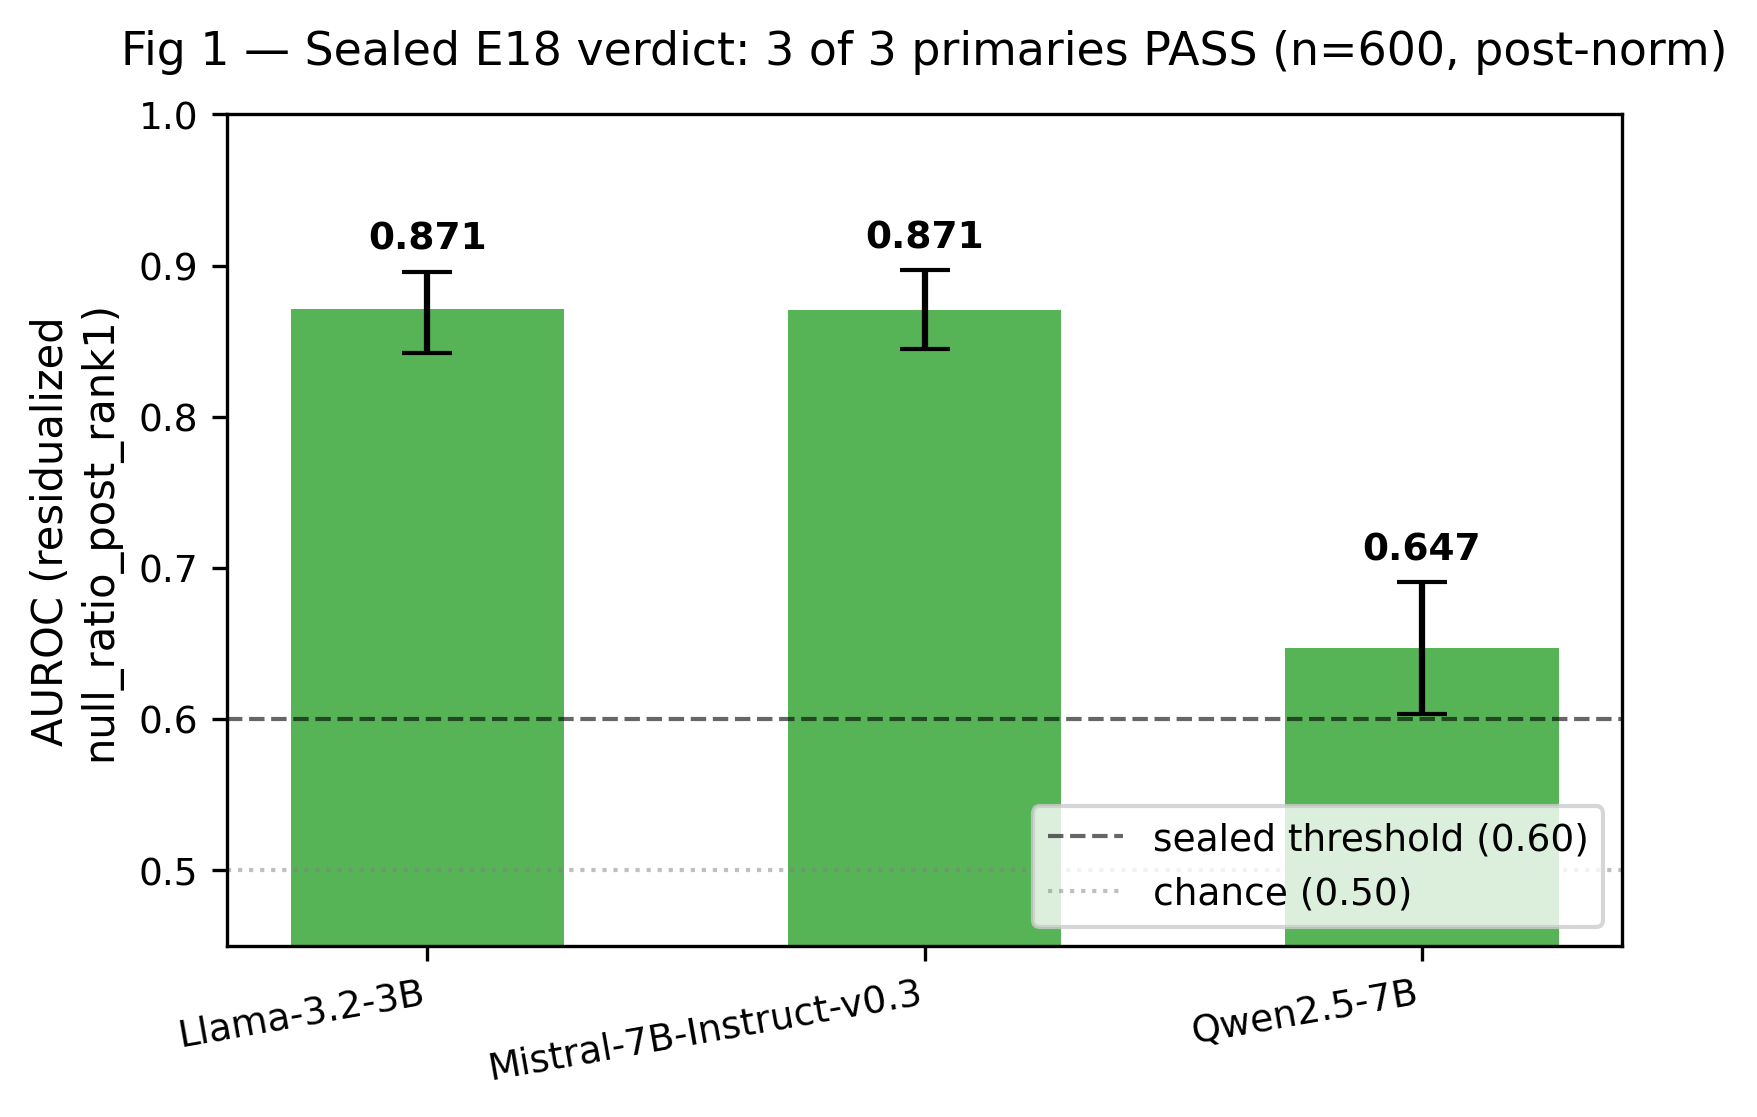
\includegraphics[width=0.7\linewidth]{pri-figures/fig1_sealed_e18.png}
  \caption{Sealed E18 magnitude-independence gate at $n=600$ per
  primary, $\Jn$-corrected post-norm geometry. AUROC of
  \texttt{null\_ratio\_post\_rank1} residualized against
  \texttt{d\_F\_lowrank32} via OLS. Error bars are 1000-sample paired
  bootstrap 95\% CIs (seed $= 20260423$). All three primaries clear
  the sealed threshold ($0.60$, dashed) with non-overlap CI vs.\ $0.5$
  (chance, dotted). Sealed bar is 2-of-3; we clear 3-of-3.}
  \label{fig:e18}
\end{figure}

All three primaries clear the $\auroc \geq 0.60$ threshold with
non-overlap 95\% CI vs.\ $0.5$. Sealed bar is 2-of-3; we clear 3-of-3.
Bootstrap CIs are $\sim 33\%$ tighter than the $n=200$ prelim
(run-02), consistent with $\sqrt{3}$ narrowing for $3\times$ more data.
Verdict structure replicates the prelim direction-for-direction.

\subsection{Sealed E17b verdict on Qwen 2.5 --- PASS}
\label{sec:results:e17b}

\begin{table}[h]
  \centering
  \small
  \begin{tabular}{lcccc}
  \toprule
  Reading & Fisher (sign) & Raw (sign) & $\Doriented$ & 95\% CI \\
  \midrule
  Buggy 2026-04-24 (run-05) & 0.7665 ($-1$) & 0.9323 ($+1$)
    & $-0.166$ & $[-0.240, -0.098]$ \\
  \textbf{Corrected 2026-04-27 (run-09)} & \textbf{0.8967 ($+1$)}
    & 0.7396 ($-1$) & $\boldsymbol{+0.157}$ &
    $\boldsymbol{[+0.125, +0.190]}$ \\
  \bottomrule
  \end{tabular}
  \caption{Sealed E17b head-to-head on Qwen 2.5 under buggy (pre-norm
  $\dh$ on post-norm basis, before $\Jn$ correction) vs.\ corrected
  (post-norm $\dh$ on post-norm basis) geometry. Buggy reading FAILS
  with Raw decisive; corrected reading PASSES with Fisher decisive.}
  \label{tab:e17b}
\end{table}

\begin{figure}[h]
  \centering
  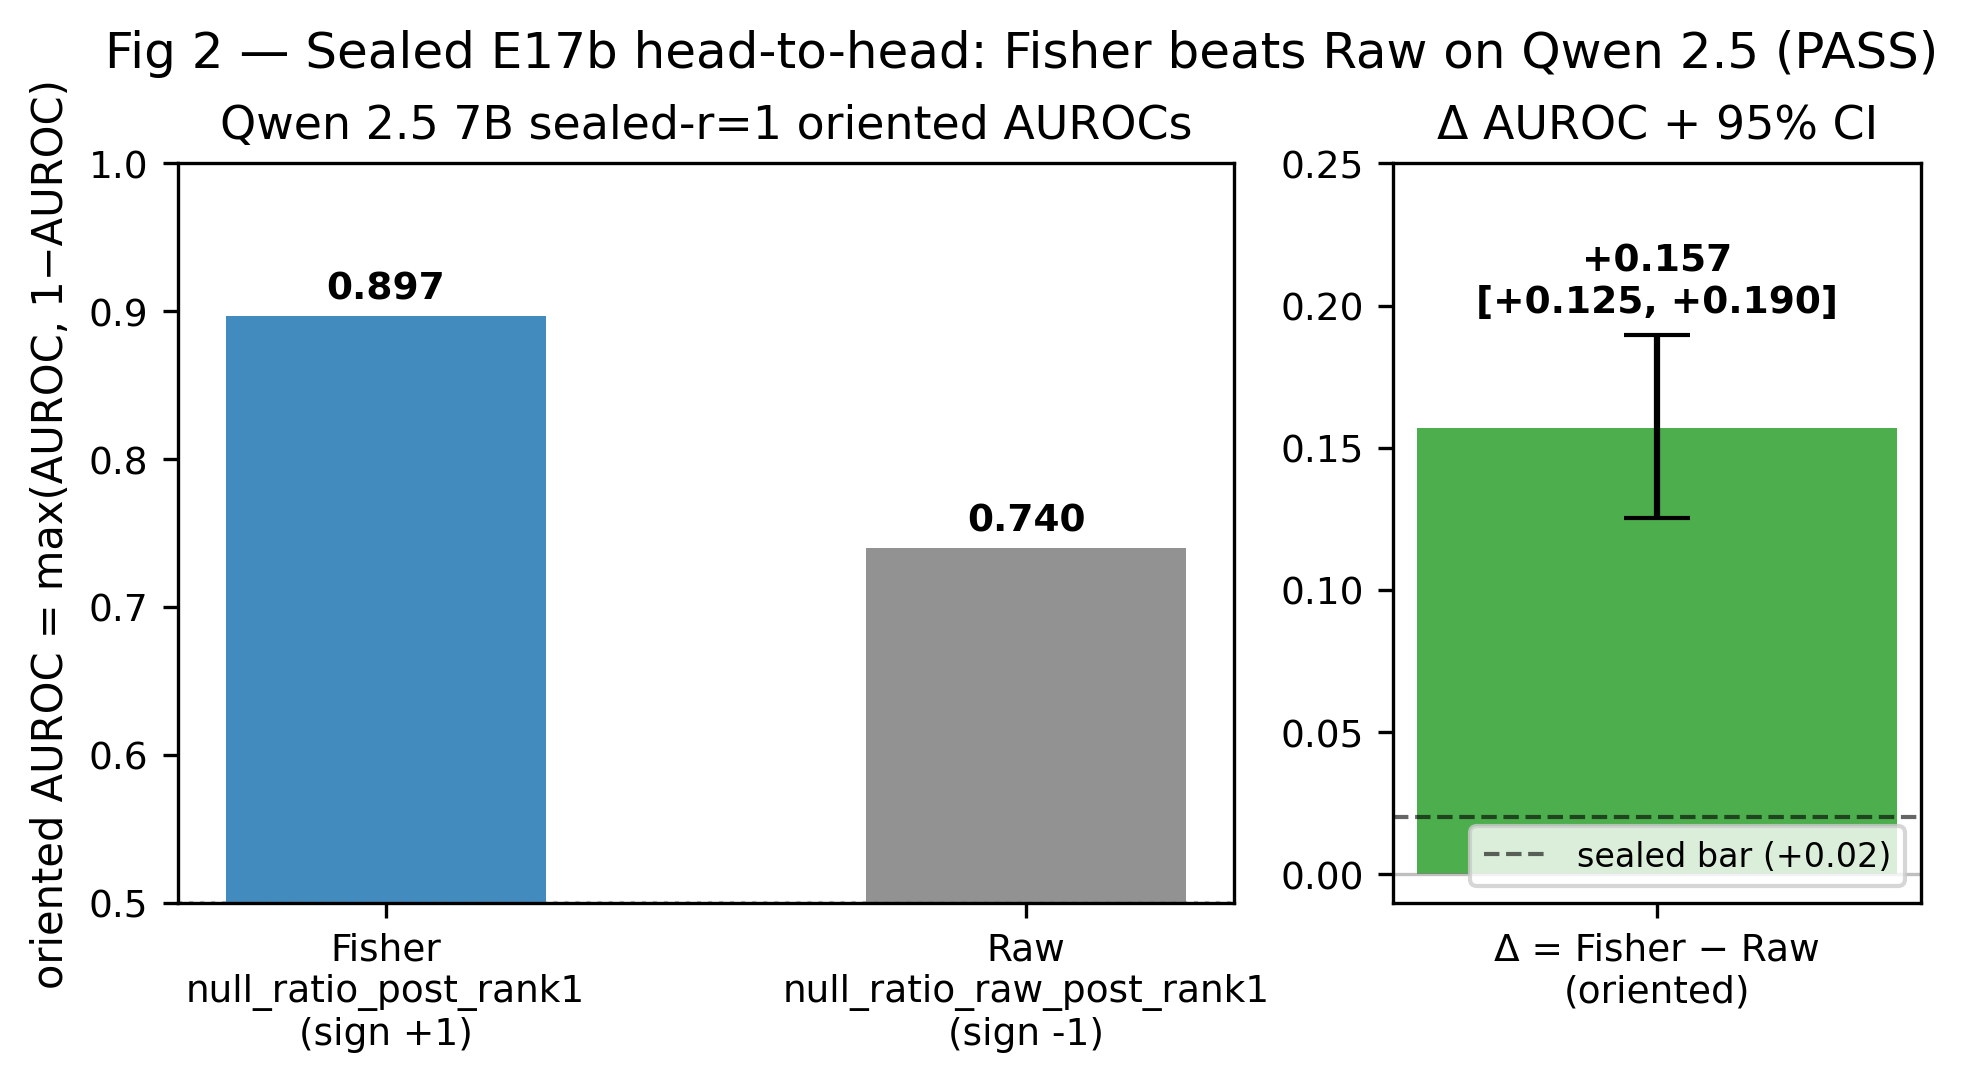
\includegraphics[width=0.85\linewidth]{pri-figures/fig2_sealed_e17b.png}
  \caption{Sealed E17b head-to-head on Qwen 2.5 7B at $n=600$.
  \textbf{Left:} oriented AUROCs of \texttt{null\_ratio\_post\_rank1}
  (Fisher, sign $+1$) and \texttt{null\_ratio\_raw\_post\_rank1} (Raw,
  sign $-1$). \textbf{Right:} $\Delta \auroc = +0.157$ $[+0.125,
  +0.190]$ (1000-sample paired bootstrap), clearing the sealed
  $+0.02$ bar (dashed) with non-overlap CI.}
  \label{fig:e17b}
\end{figure}

\begin{figure}[h]
  \centering
  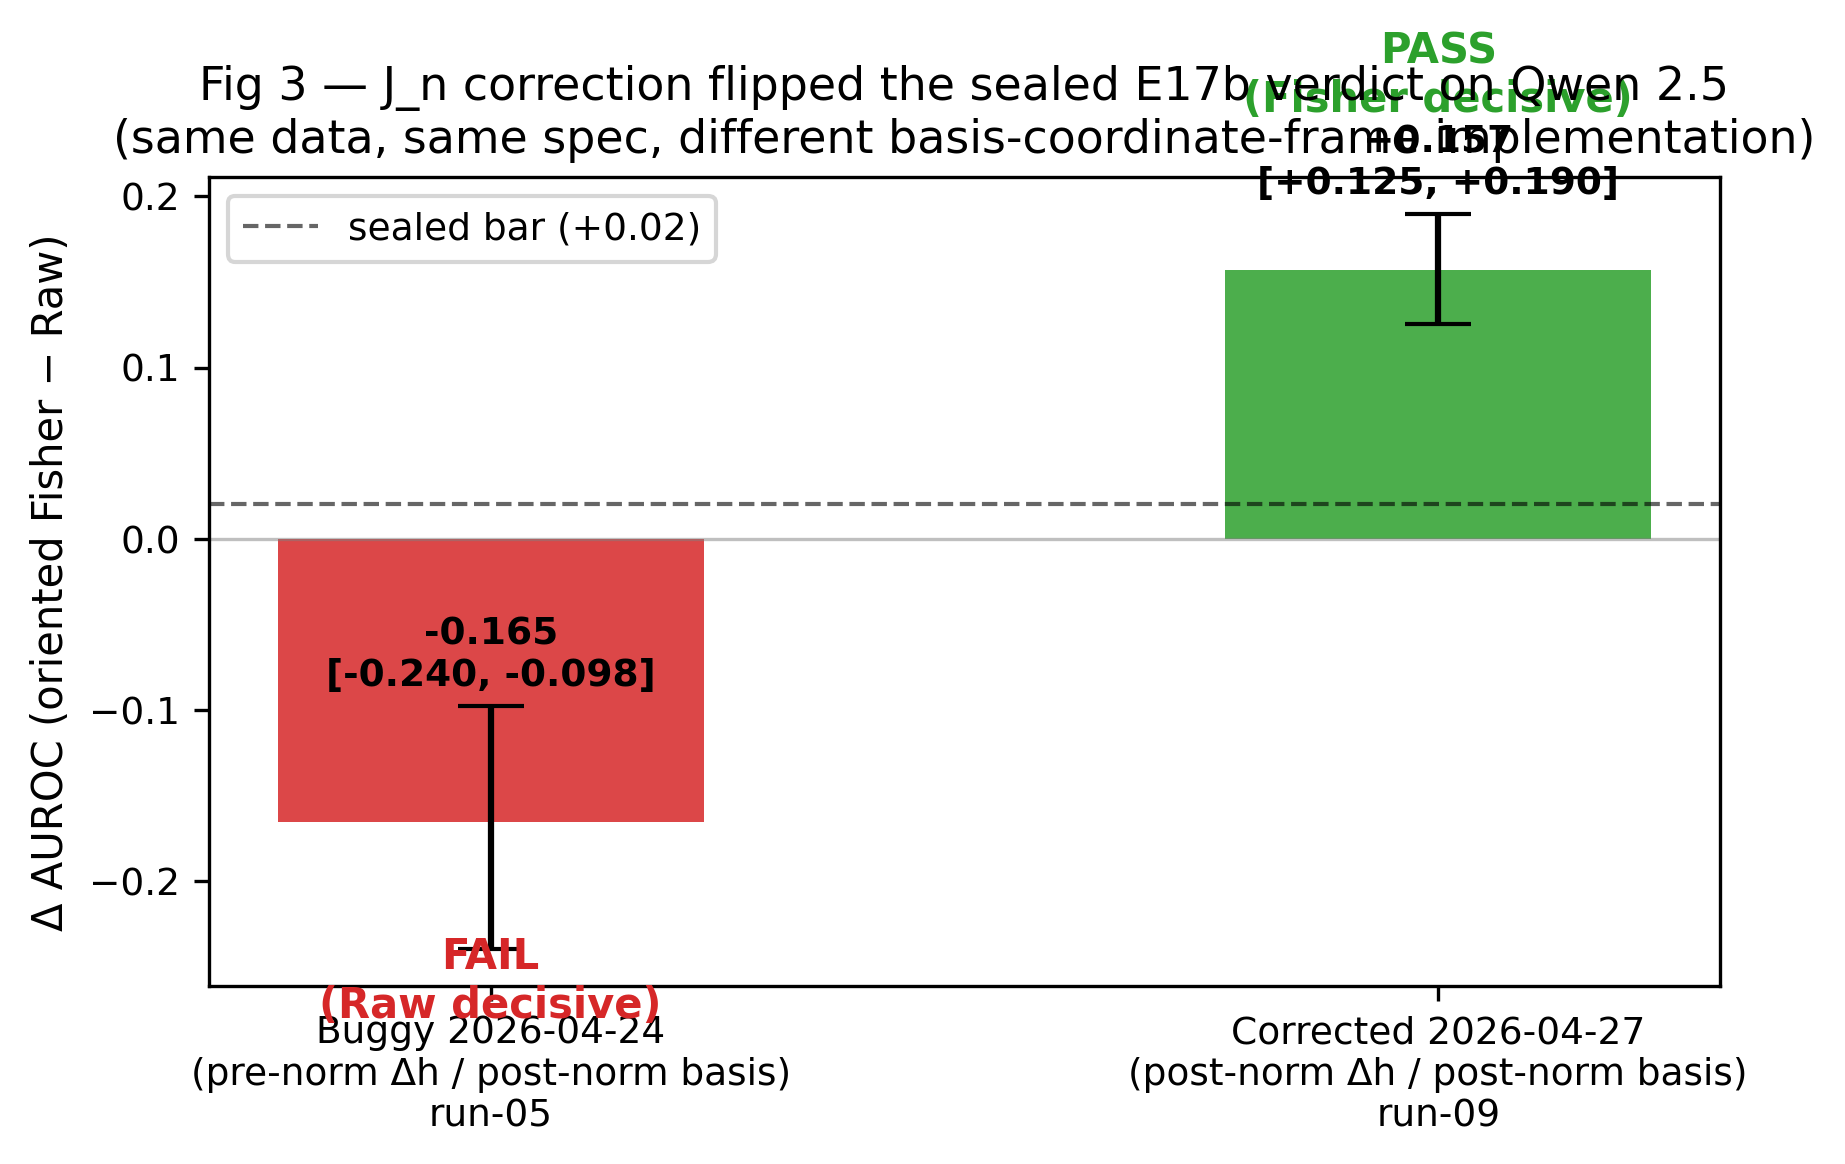
\includegraphics[width=0.75\linewidth]{pri-figures/fig3_jn_correction.png}
  \caption{$\Jn$ geometry correction effect on the sealed E17b verdict
  (Qwen 2.5). Same data, same sealed spec, different
  basis-coordinate-frame implementation. Buggy reading from
  2026-04-24 (pre-norm $\dh$ projected onto post-norm basis):
  $\Delta = -0.166$, FAIL with Raw decisive. Corrected reading from
  2026-04-27 (post-norm $\dh$ projected onto post-norm basis,
  $\Jn$-consistent): $\Delta = +0.157$, PASS with Fisher decisive.
  The $+0.32$ swing is the correction's effect on the head-to-head;
  sealed E18 (\Cref{fig:e18}) is unaffected because residualization
  absorbs the bias (\Cref{sec:methods:jn}).}
  \label{fig:jn}
\end{figure}

The Fisher-weighted basis discriminates contradictions in the
predicted direction with non-overlap CI; the static raw basis
discriminates inverted (sign $-1$) at this analysis plane. $\Delta
\auroc = +0.157$ clears the sealed $+0.02$ bar by $7.9\times$. The
$+0.32$ swing between rows in \Cref{tab:e17b} is the $\Jn$
correction's effect on the head-to-head (\Cref{sec:methods:jn}); we
report both rows for transparency. The corrected reading replicates
the $n=200$ prelim ($+0.150$ $[+0.100, +0.201]$) within bootstrap
noise, with CI tightened by $\sim 34\%$ as expected for the $3\times$
sample-size increase.

\subsection{Cross-architecture motifs}
\label{sec:results:motifs}

We compute the head-to-head $\Doriented$ across all 6 models, all 13
ranks in the sweep, both pooled and chain-length-stratified at $n=300$
per stratum. The $6\times 13\times 2 = 156$-cell landscape exposes
three structurally distinct architecture-dependence motifs.

\begin{figure}[h]
  \centering
  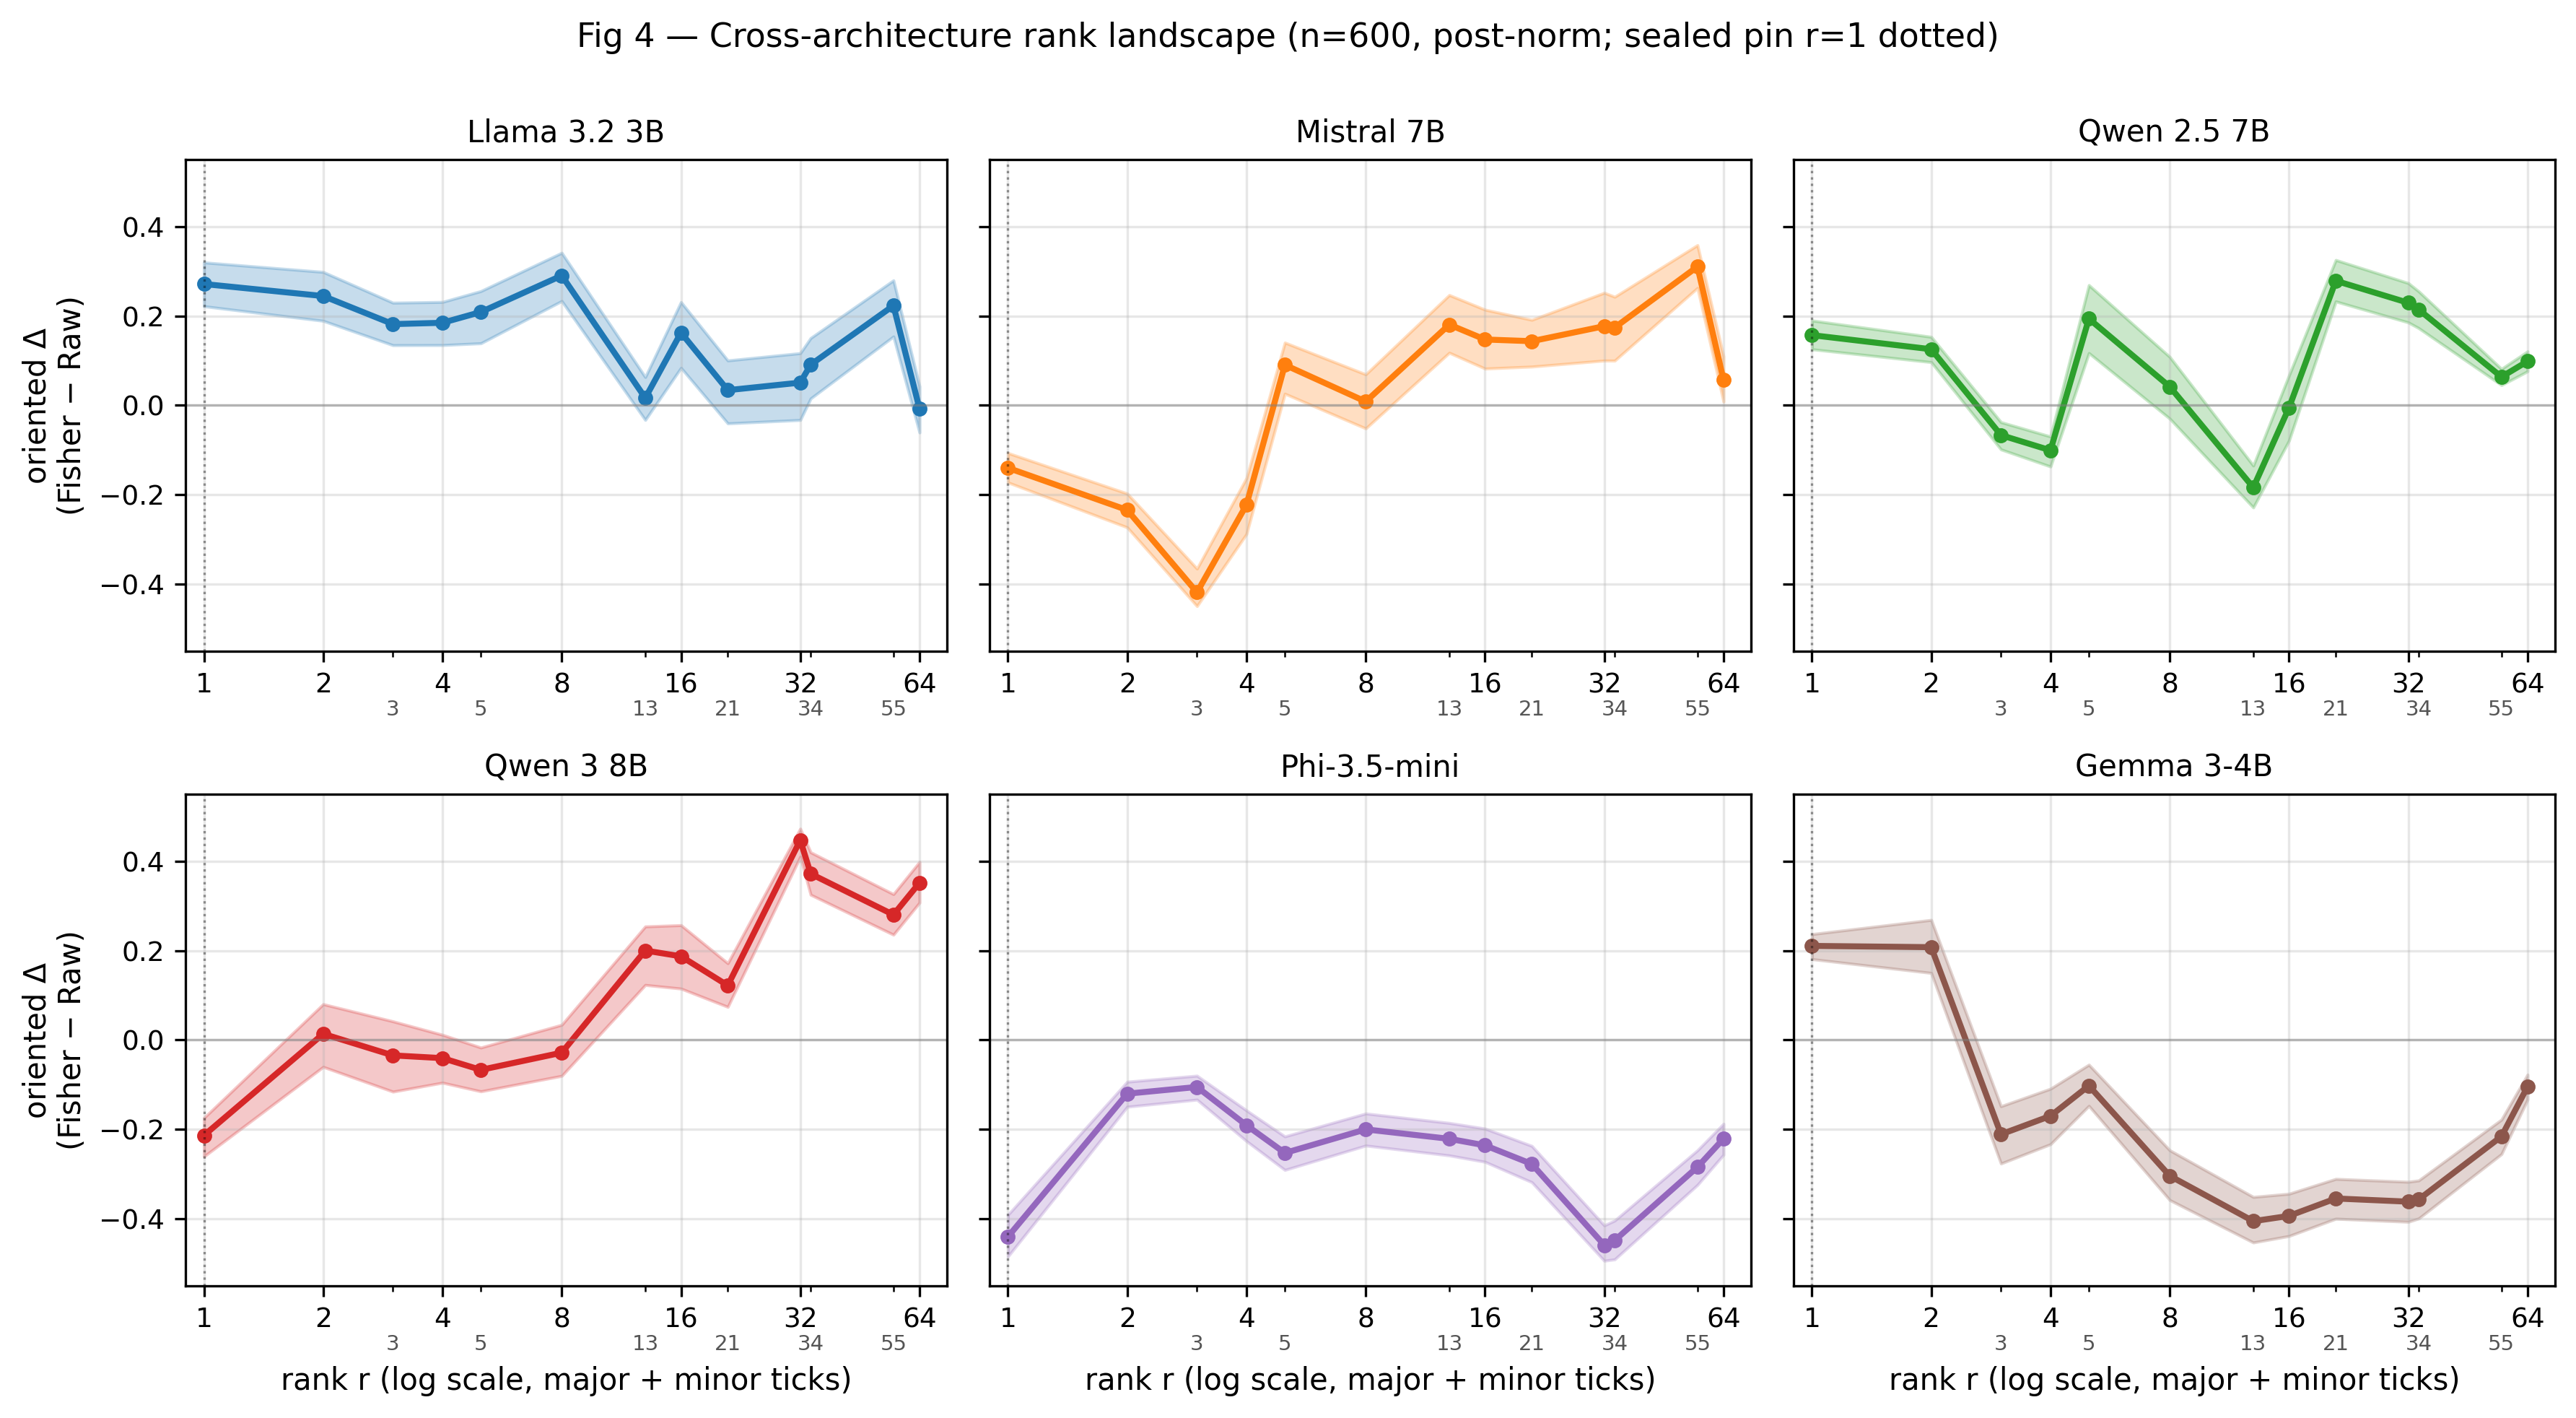
\includegraphics[width=\linewidth]{pri-figures/fig4_rank_landscape.png}
  \caption{Cross-architecture rank landscape at $n=600$. Each panel
  shows $\Doriented$ (Fisher $-$ Raw) vs.\ rank (log scale, major
  ticks at $1, 2, 4, 8, 16, 32, 64$; minor ticks at $3, 5, 13, 21, 34,
  55$) for one model, with 1000-sample bootstrap 95\% CI bands.
  Sealed pin $r=1$ marked as a dotted vertical. $\Delta > 0$ = Fisher
  decisive; $\Delta < 0$ = Raw decisive. Llama is Fisher-or-tied
  throughout. Mistral flips Raw $\to$ Fisher at $r=4 \to r=5$.
  Qwen 2.5 oscillates F $\to$ R $\to$ F $\to$ R $\to$ F. Qwen 3 is
  Raw at sealed $r=1$, Fisher decisive from $r=13$ onward (peak
  $+0.447$ at $r=32$). Phi-3.5-mini is stable Raw across all 13
  ranks (Motif 1). Gemma 4B flips F $\to$ R sharply at $r=2 \to r=3$
  (Motif 2).}
  \label{fig:landscape}
\end{figure}

\subsubsection{Motif 1 --- Stable Raw across all 13 ranks (Phi-3.5-mini)}

\begin{table}[h]
  \centering
  \footnotesize
  \begin{tabular}{lccccccccccccc}
  \toprule
  rank & 1 & 2 & 3 & 4 & 5 & 8 & 13 & 16 & 21 & \textbf{32} & 34 & 55 & 64 \\
  \midrule
  $\Delta$ & $-0.441$ & $-0.120$ & $-0.105$ & $-0.191$ & $-0.253$
    & $-0.200$ & $-0.221$ & $-0.236$ & $-0.278$ & $\boldsymbol{-0.459}$
    & $-0.449$ & $-0.285$ & $-0.221$ \\
  \bottomrule
  \end{tabular}
  \caption{Phi-3.5-mini $\Doriented$ across the rank sweep at $n=600$
  pooled. Raw decisive (negative $\Delta$) at every rank. Peak
  Raw-margin at $r=32$.}
  \label{tab:phi}
\end{table}

Phi-3.5-mini is the only model in the lineup with Raw decisive at
every single rank in the sweep, every chain-length stratum.
\texttt{null\_ratio\_raw\_post\_rank1} $= 0.9989$ --- nearly perfect
contradiction discrimination via the static $\Wu$ SVD basis alone.
\textbf{Phi is the canonical ``HARP-style detection works as
advertised'' architecture, and the headline counter-example to
``Fisher pullback uniformly wins.''} The static basis carries the
rupture signal so cleanly that Fisher's per-sample reweighting cannot
add.

\subsubsection{Motif 2 --- Within-model rank flip robust to chain
length (Gemma 3-4B)}

\begin{figure}[h]
  \centering
  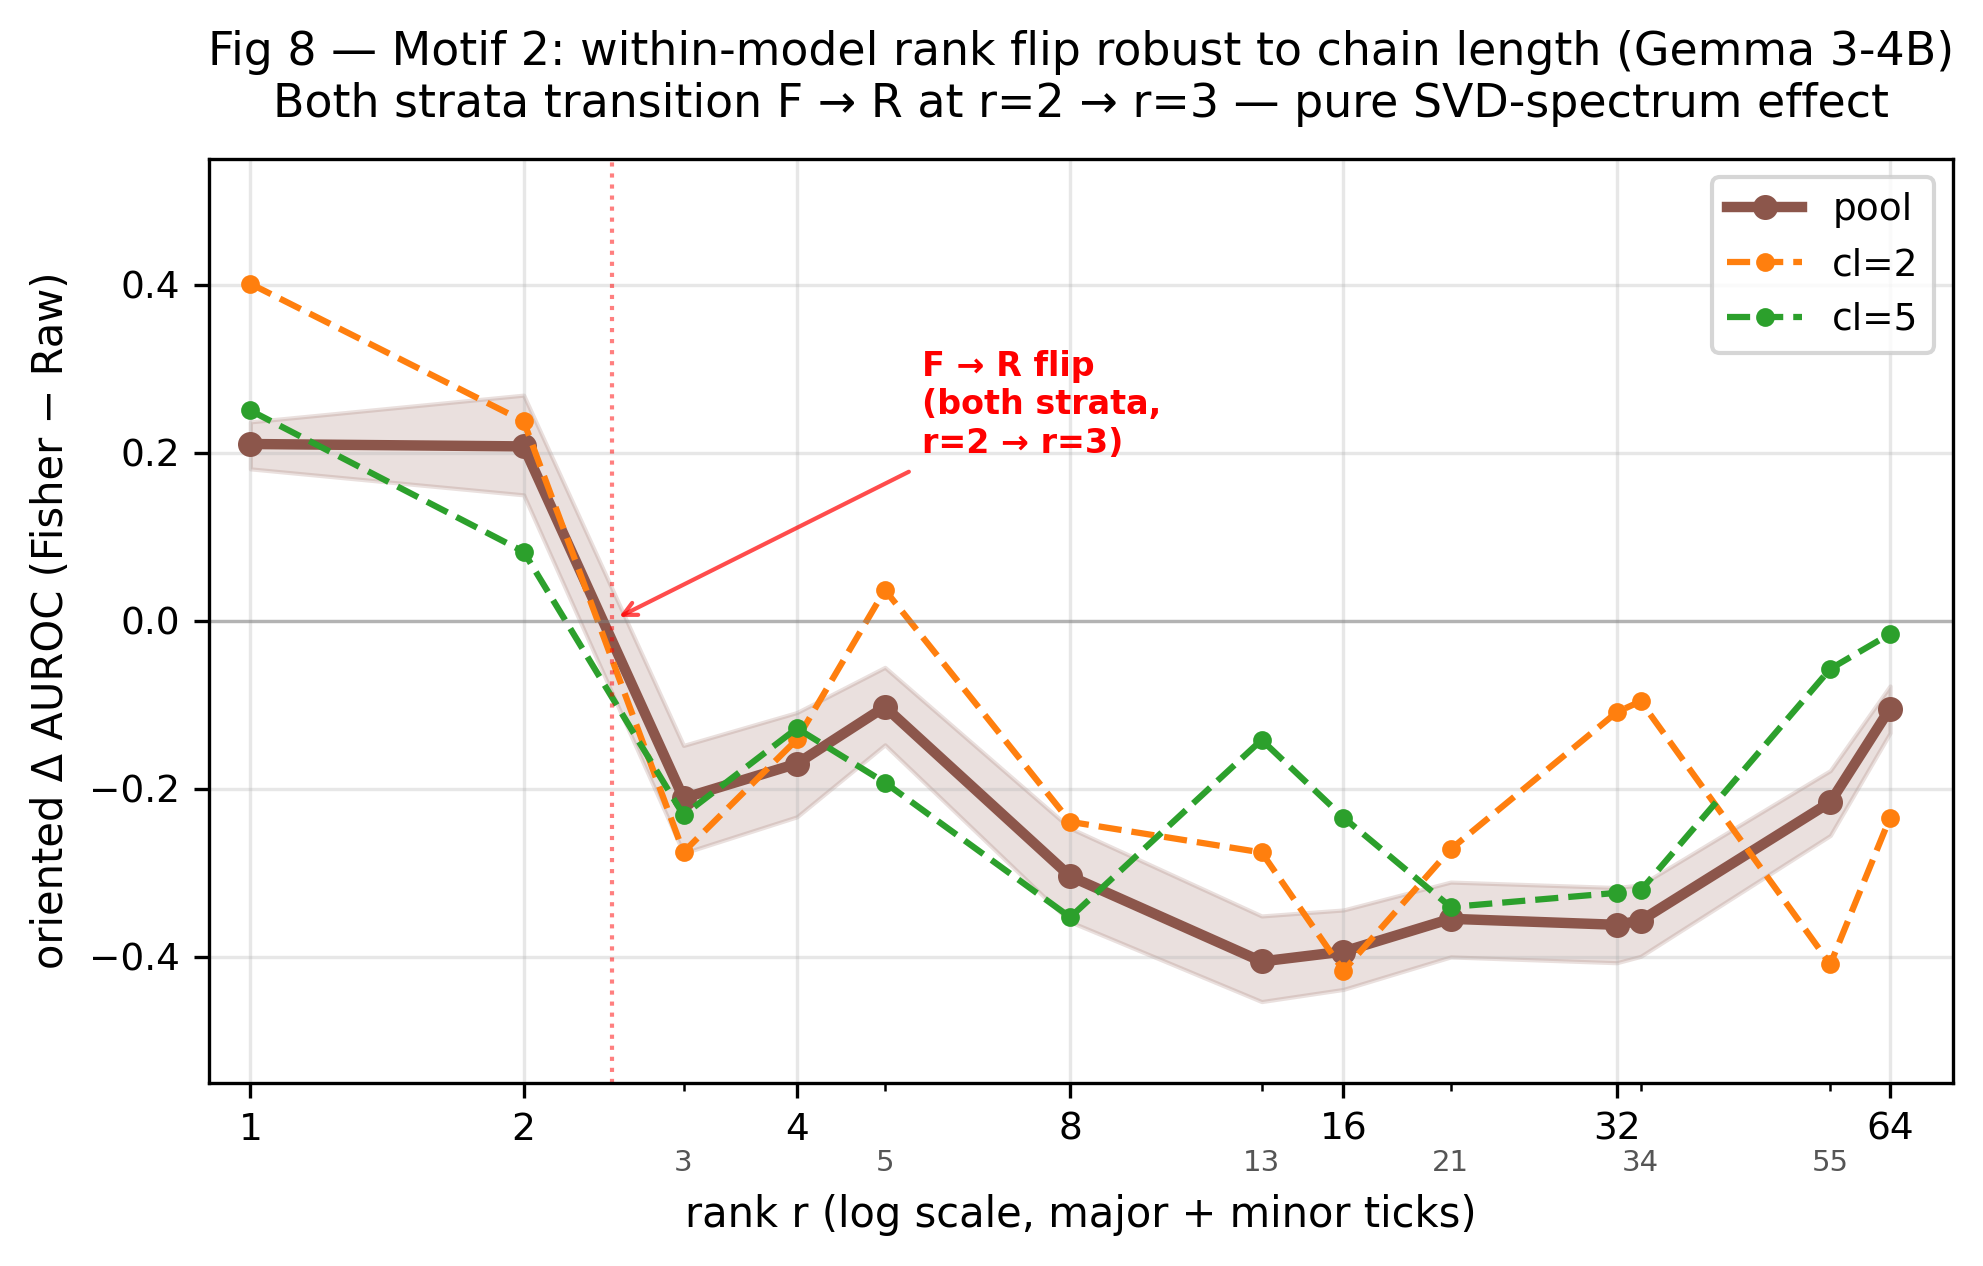
\includegraphics[width=0.85\linewidth]{pri-figures/fig8_gemma_rankflip.png}
  \caption{Motif 2 --- within-model rank flip robust to chain length
  (Gemma 3-4B). Three lines: pool ($n=600$, solid brown), cl$=$2
  stratum ($n=300$, dashed orange), cl$=$5 stratum ($n=300$, dashed
  green). Both chain-length strata transition F $\to$ R together at
  $r=2 \to r=3$ (red dotted vertical). The flip is a property of the
  SVD spectrum, not a chain-length artifact.}
  \label{fig:gemma}
\end{figure}

The flip from Fisher to Raw is sharp at $r=2 \to r=3$: pool
$\Doriented$ goes from $+0.207$ (Fisher decisive at non-overlap CI)
to $-0.211$ (Raw decisive at non-overlap CI) within one rank step.
\textbf{Both chain-length strata show the same $r=2 \to r=3$
transition} (one borderline tie at $r=5$ / cl$=$2). The flip is a
property of the SVD spectrum, not a chain-length artifact --- pure
rank-axis architecture-dependence. The sealed pin at $r=1$ picks up
Fisher; pinning $r=32$ would have picked up Raw on the same data ---
operationalizing the methodological point that the rank choice is a
methodological commitment, not a free parameter.

\subsubsection{Motif 3 --- Chain-length $\times$ rank interaction with
two Simpson's-paradox sites (Mistral 7B)}

\begin{table}[h]
  \centering
  \small
  \begin{tabular}{cccrr}
  \toprule
  rank & pool $\Delta$ & cl$=$2 $\Delta$ & cl$=$5 $\Delta$ &
    $\Dcross$ (cl$=$2 $-$ cl$=$5) \\
  \midrule
  $\boldsymbol{1}$  & $\boldsymbol{R\ -0.140}$
    & $\boldsymbol{F\ +0.065}$ [+0.041, +0.093] & $\cdot\ +0.002$
    & $+0.062$ \\
  $4$  & $R\ -0.223$ & $R\ -0.097$ & $R\ -0.383$ & $+0.287$ \\
  $13$ & $F\ +0.181$ & $F\ +0.208$ & $\cdot\ -0.002$ & $+0.210$ \\
  $21$ & $F\ +0.144$ & $F\ +0.101$ & $R\ -0.133$ & $+0.234$ \\
  $\boldsymbol{32}$ & $\boldsymbol{F\ +0.177}$
    & $\boldsymbol{R\ -0.196}$ [-0.262, -0.131]
    & $\boldsymbol{F\ +0.379}$ [+0.319, +0.450]
    & $\boldsymbol{-0.575}$ \\
  $34$ & $F\ +0.174$ & $R\ -0.204$ & $F\ +0.357$ & $-0.561$ \\
  $55$ & $F\ +0.310$ & $F\ +0.174$ & $F\ +0.228$ & $-0.053$ \\
  \bottomrule
  \end{tabular}
  \caption{Mistral 7B $\Doriented$ across selected ranks at $n=600$
  pool / $n=300$ per chain-length stratum. F $=$ Fisher decisive,
  R $=$ Raw decisive, $\cdot$ $=$ tie (CI straddles zero). The two
  Simpson's-paradox sites are at $r=1$ and $r=32$ (boldface). At
  $r=32$ both stratum CIs are non-overlapping in opposite directions;
  $\Dcross = -0.575$ is the largest cross-stratum spread observed in
  the entire 156-cell grid.}
  \label{tab:mistral}
\end{table}

\begin{figure}[h]
  \centering
  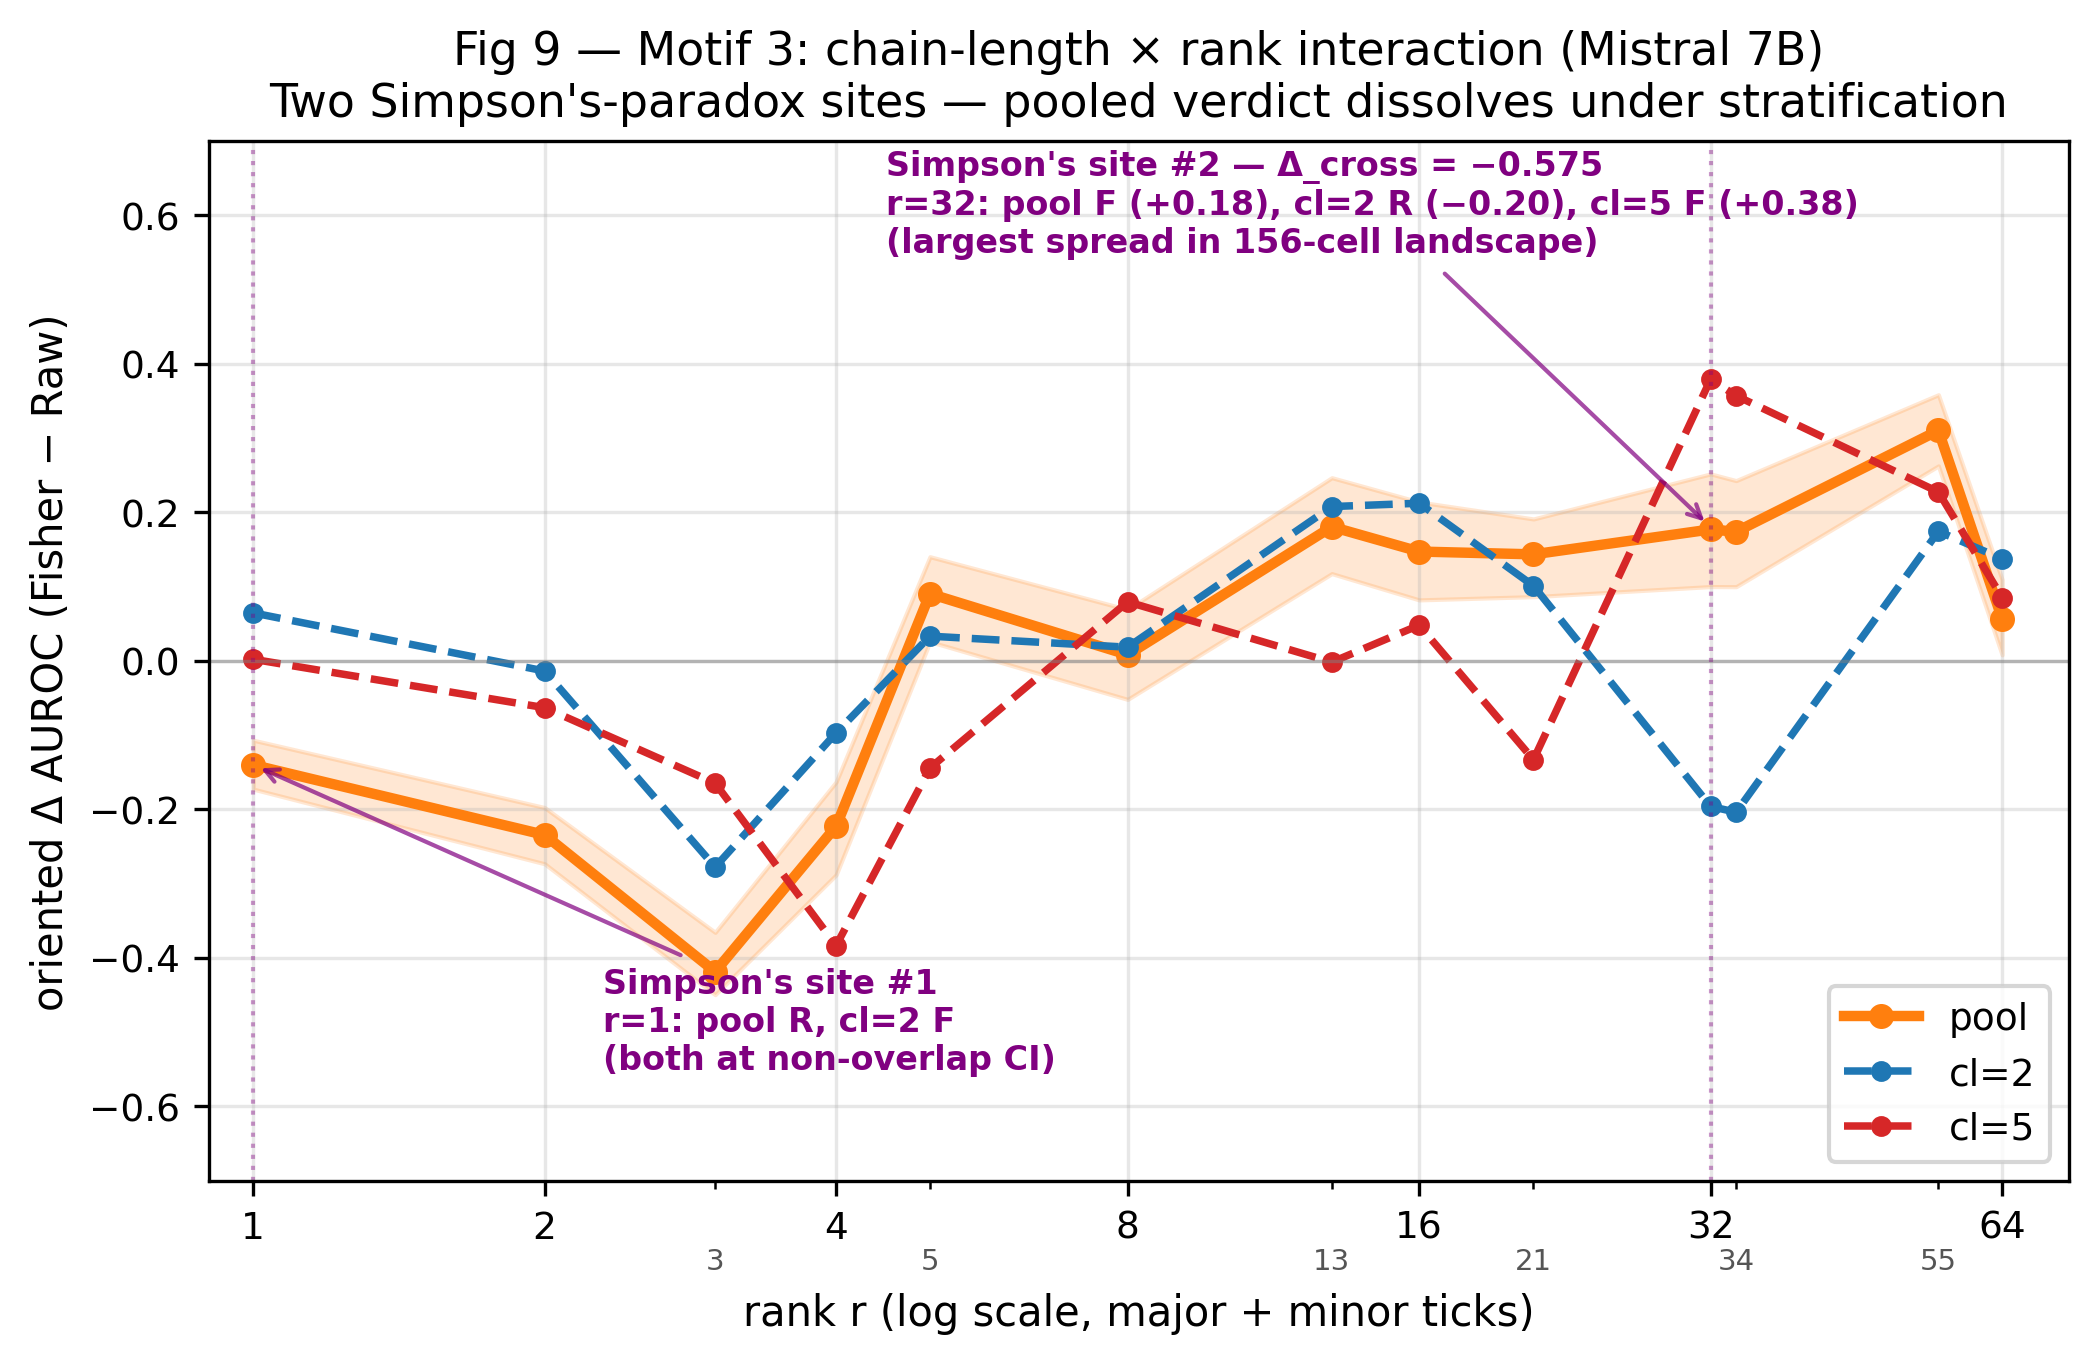
\includegraphics[width=0.95\linewidth]{pri-figures/fig9_mistral_simpsons.png}
  \caption{Motif 3 --- chain-length $\times$ rank interaction
  (Mistral 7B). Same three-line layout as \Cref{fig:gemma}: pool
  ($n=600$, solid orange), cl$=$2 ($n=300$, dashed blue), cl$=$5
  ($n=300$, dashed red). Two purple dotted verticals mark the
  Simpson's-paradox sites at $r=1$ and $r=32$. \textbf{Site \#1
  ($r=1$):} pool Raw-decisive ($-0.140$) but cl$=$2 Fisher-decisive
  ($+0.065$) and cl$=$5 tied --- pool's Raw is a mixing artifact.
  \textbf{Site \#2 ($r=32$):} pool Fisher-decisive ($+0.177$) but
  cl$=$2 Raw-decisive ($-0.196$) and cl$=$5 Fisher-decisive
  ($+0.379$), with both stratum CIs non-overlapping in opposite
  directions --- $\Dcross = -0.575$, the largest cross-stratum spread
  observed in the entire 156-cell model $\times$ rank $\times$
  chain\_length grid.}
  \label{fig:mistral}
\end{figure}

Mistral has \textbf{two Simpson's-paradox sites at non-overlap CI:}
\begin{itemize}[leftmargin=*, itemsep=2pt, topsep=2pt]
  \item \textbf{At sealed $r=1$:} the pool says Raw decisive ($\Delta
  = -0.140$), but the stratum-level reading is Fisher decisive at
  cl$=$2 ($+0.065$ $[+0.041, +0.093]$, CI fully positive) and tied at
  cl$=$5 ($+0.002$ $[-0.022, +0.028]$). Mistral is \textbf{never
  Raw-decisive at the stratum level} --- the pooled ``Raw'' verdict
  is a mixing artifact of two chain-length subgroups whose Fisher
  and Raw discrimination axes have different orientations.
  \item \textbf{At $r=32$--$34$:} the pool says Fisher decisive, but
  cl$=$2 reads Raw decisive ($-0.196$) and cl$=$5 reads Fisher
  decisive ($+0.379$), both at non-overlap 95\% CI in opposite
  directions. \textbf{$\Dcross = -0.575$ at $r=32$ is the largest
  cross-stratum spread observed across all 156 cells in the model
  $\times$ rank $\times$ chain-length grid.}
\end{itemize}

Other architectures' cross-stratum spreads stay within $\pm 0.3$ at
every rank in the sweep. Mistral is the unique flag-bearer for
chain-length-coupled rupture geometry. The mechanistic hypothesis
(\Cref{sec:disc:mechanism}): Mistral writes a newline at gen\_step$=$1
(``begin the answer block'') rather than committing to actual answer
content; the newline's geometric position relative to the
contradiction event in token-space shifts dramatically with chain
depth.

\paragraph{Pooled cross-architecture summary.}
At the sealed rank$=$1 plane, the six architectures partition as:

\begin{itemize}[leftmargin=*, itemsep=2pt, topsep=2pt]
  \item \textbf{Fisher decisive (3):} Llama 3.2 3B
  ($\Delta = +0.272$ $[+0.222, +0.320]$), Qwen 2.5 7B sealed
  ($+0.157$ $[+0.125, +0.190]$), Gemma 3-4B ($+0.210$ $[+0.181,
  +0.237]$).
  \item \textbf{Raw decisive (3):} Mistral 7B
  ($\Delta = -0.140$ $[-0.173, -0.107]$), Qwen3 8B
  ($-0.214$ $[-0.261, -0.175]$), Phi-3.5-mini
  ($-0.441$ $[-0.485, -0.392]$).
\end{itemize}

Cross-generation within Qwen-family (2.5 Fisher $\to$ 3 Raw) and
within-vendor (Llama Fisher vs.\ Mistral Raw) both flip; vendor and
parameter-count are not predictive.

\subsection{Baselines}
\label{sec:results:baselines}

\begin{table}[h]
  \centering
  \small
  \begin{tabular}{lccccc}
  \toprule
  Primary & surprise & PRI v1 cosine & PRI v2 topk32 & PRI v2 lowrank32
    & v3 sealed \\
  \midrule
  Llama 3.2 3B  & 0.6347 & 0.6224 & 0.7528 & 0.7500 & 0.8975 \\
  Mistral 7B    & 0.5187 & 0.5309 & 0.6623 & 0.6618 & 0.7849 \\
  Qwen 2.5 7B   & 0.8947 & 0.9155 & 0.7906 & 0.7948 & 0.8967 \\
  \bottomrule
  \end{tabular}
  \caption{Baseline AUROCs on the sealed primaries at $n=600$. v3
  sealed = \texttt{null\_ratio\_post\_rank1}. The sealed v3 metric
  outperforms PRI v1 and v2 on Llama and Mistral by clear margins. On
  Qwen 2.5, surprise (0.8947) and PRI v1 cosine (0.9155) are
  competitive with the sealed v3 metric (0.8967) --- one of the
  model-specific anomalies worth flagging in
  \Cref{sec:disc:mechanism}.}
  \label{tab:baselines}
\end{table}

% =====================================================================
\section{Discussion}
\label{sec:discussion}

\subsection{Why architecture-dependence rather than universal Fisher
win}
\label{sec:disc:mechanism}

The qualitative content of the gen\_step$=$1 token differs across
architectures, and so does the alignment of $\Wu$'s top-1 right
singular vector $V_\text{raw}[0]$. We characterized both empirically
on $N=100$ stratified puzzles per model (50 ctrl $\times$ 50 contr
$\times$ 2 chain lengths, seed $= 20260423$), under $\Jn$-corrected
post-norm geometry. \Cref{tab:wu_axis} reports, per model: the modal
gen\_step$=$1 commit token; $V_\text{raw}[0]$'s top-3 positive and
top-3 negative tokens; targeted projections of YES / NO / \texttt{\textbackslash n}
onto $V_\text{raw}[0]$; and per-sample signed
$\dh_\text{Jn} \cdot V_\text{raw}[0]$ for ctrl vs.\ contr.

\begin{table*}[t]
  \centering
  \scriptsize
  \resizebox{\linewidth}{!}{%
  \begin{tabular}{lllllrrrcc}
  \toprule
  Model & modal commit & $V_\text{raw}[0]$ top-3 pos & $V_\text{raw}[0]$ top-3 neg & ` YES' & ` NO' & \texttt{\textbackslash n} & ctrl mean$\pm$std & contr mean$\pm$std & $\Delta$ \\
  \midrule
  Llama 3.2 3B & ` Answer' (98\%) & \texttt{,}\ \texttt{`\ '}\ \texttt{`\ ('} & \texttt{SCRI}\ \texttt{using}\ \texttt{TRGL} & $-0.338$ & $-0.088$ & $+0.576$ & $+1.30 \pm 0.15$ & $+1.36 \pm 0.26$ & $+0.062$ \\
  Mistral 7B & \texttt{\textbackslash n} (100\%) & \texttt{(}\ \texttt{\textbackslash n}\ \texttt{and} & \texttt{qpoint}\ \texttt{ICENSE}\ \texttt{ityEngine} & $+0.034$ & $-0.028$ & $+0.127$ & $+3.01 \pm 0.41$ & $+4.64 \pm 0.52$ & $+1.632$ \\
  Qwen 2.5 7B & ` NO' (52\%) & \texttt{`\ '}\ \texttt{,}\ \texttt{1} & \texttt{.IsNullOr}\ \texttt{`\ volunte'}\ \texttt{gnore} & $-0.104$ & $+0.051$ & $+0.543$ & $-0.30 \pm 9.94$ & $-18.70 \pm 1.33$ & $-18.400$ \\
  Qwen3 8B & ` Answer' (79\%) & \texttt{`\ neighb'}\ \texttt{`\ porno'}\ \texttt{`\ somew'} & \texttt{`\ '}\ \texttt{\textbackslash n}\ \texttt{,} & $+0.352$ & $-0.072$ & $-1.335$ & $+0.77 \pm 0.40$ & $-1.57 \pm 2.55$ & $-2.336$ \\
  Phi-3.5-mini & \texttt{\textbackslash n} (100\%) & \texttt{provin}\ \texttt{Wikip}\ \texttt{zna} & \texttt{(}\ \texttt{\textbackslash n}\ \texttt{in} & --- & $+0.344$ & $-0.469$ & $-9.57 \pm 0.59$ & $-8.14 \pm 0.89$ & $+1.434$ \\
  Gemma 3-4B & \texttt{\textbackslash n} (100\%) & \texttt{S}\ \texttt{(}\ \texttt{g} & \texttt{`\ ('}\ \texttt{\textbackslash n}\ \texttt{\textbackslash n\textbackslash n} & --- & $+0.029$ & $-0.329$ & $-6.09 \pm 0.68$ & $-6.15 \pm 0.49$ & $-0.061$ \\
  \bottomrule
  \end{tabular}%
  }
  \caption{Cross-model $\Wu$ top-1 axis character at gen\_step$=$1.
  Targeted projection columns (` YES', ` NO', \texttt{\textbackslash n})
  give signed $W_u[t] \cdot V_\text{raw}[0]$ for the indicated single
  token. ``---'' denotes that the indicated string does not encode to
  a single token in this tokenizer. Right two columns are per-sample
  signed $\dh_\text{Jn} \cdot V_\text{raw}[0]$ across $N=100$
  stratified puzzles. $\Delta = \text{contr} - \text{ctrl}$. Source:
  \texttt{scripts/diagnostics/diagnose\_raw\_top1.py},
  \texttt{2026-04-30}.}
  \label{tab:wu_axis}
\end{table*}

Three observations restructure the architecture-dependence story.

\paragraph{1. gen\_step$=$1 commit splits 3/3 (newline / content), but
does not predict Fisher-vs-Raw.} Mistral, Phi, and Gemma 4B all commit
\texttt{\textbackslash n} at 100\% of samples; Llama, Qwen 2.5, and
Qwen3 commit \texttt{` Answer'}-class tokens at 52--98\%. The earlier
``newline-commit $\Rightarrow$ Raw'' / ``content-commit $\Rightarrow$
Fisher'' partition fits 4 of 6 (Mistral$+$Phi $\to$ Raw,
Llama$+$Qwen 2.5 $\to$ Fisher) but Gemma 4B (newline-commit,
Fisher-decisive) and Qwen3 (content-commit, Raw-decisive) break it.
The commit token alone is not the load-bearing variable.

\paragraph{2. What does predict Fisher-vs-Raw is the discriminative
strength of $V_\text{raw}[0]$ itself.} Two architectures (Mistral, Phi)
have strong same-sign rupture-magnitude separation on $V_\text{raw}[0]$
--- ctrl and contr both project on one side of the axis, magnitude
separates them, and Cohen's-$d$-equivalents are large ($\approx 3.5$
for Mistral, $\approx 1.9$ for Phi). Their static $\Wu$ top-1 SVD
direction \emph{happens to encode rupture magnitude} relative to the
model's commit, so $\textsc{Raw}_\text{post,rank=1}$ saturates ($0.99$
on Mistral, $0.9989$ on Phi) and Fisher's per-sample reweighting cannot
add. Two architectures (Llama, Gemma 4B) have $V_\text{raw}[0]$
discrimination near zero ($|\Delta| < 0.07$, $d \approx 0.1$--$0.3$),
and Fisher's reweighting recovers the signal that the static basis
misses. The remaining two (Qwen 2.5, Qwen3) sit between:
$V_\text{raw}[0]$ carries discriminative signal but with high
within-class variance (Qwen 2.5 ctrl std $= 9.94$ vs.\ Mistral $0.41$)
or sign-split distributions, leaving headroom for Fisher to refine
the basis.

\paragraph{3. Mistral and Phi share a non-content rupture-magnitude
axis despite different vendors and tokenizers.} Mistral's
$V_\text{raw}[0]$ top tokens are code-domain fragments
(\texttt{qpoint}, \texttt{ICENSE}, \texttt{ityEngine}) plus common
short tokens; Phi's are European-language fragments (\texttt{provin},
\texttt{Wikip}, \texttt{Magyar}) plus common short tokens. Neither is
a YES/NO bipolar axis; both have \texttt{\textbackslash n} as a strong
projection (Mistral $+0.13$, Phi $-0.47$). The shared structure is not
``what $V_\text{raw}[0]$ points at''~--- it is \emph{that}
$V_\text{raw}[0]$ is anchored to the structural commit
(\texttt{\textbackslash n}) rather than to answer content,
\emph{and} that $\dh_\text{Jn}$ at the commit moment lands monotonically
on $V_\text{raw}[0]$. The two models converge on the same regime (Raw
saturation) via two different vocabulary-specific top-token signatures.

The cross-stratum interpretation in
\Cref{sec:results:motifs} still holds for Mistral
specifically~--- chain-length couples to where the
\texttt{\textbackslash n}-commit lands relative to the
contradiction event in token-space, producing the
$\Dcross = -0.575$ spread at $r=32$. But the universal
``newline-commit decouples~$\leftrightarrow$ content-commit decouples''
claim in earlier drafts was an over-fit; chain-length coupling can in
principle exist on any architecture whose commit is structural rather
than content-bearing. Phi's chain-length sensitivity at the same plane
is a follow-up worth checking explicitly.

A universal pattern across all six models corroborates the
chain-length mechanism: \textbf{$|\Doriented|$ is sharper at cl$=$2
than cl$=$5} at sealed $r=1$ (Llama $0.397$ vs.\ $0.170$; Mistral
$0.065$ vs.\ $0.002$; Qwen 2.5 $0.138$ vs.\ $0.063$; Qwen3 $-0.317$
vs.\ $-0.167$; Phi $-0.374$ vs.\ $-0.228$; Gemma 4B $0.401$ vs.\
$0.250$). Short reasoning chains amplify the Fisher-vs-Raw
discrimination signal; long chains diffuse it. The rupture geometry is
most informative when the commit and the contradiction are close in
token-space.

The Qwen 2.5 baseline anomaly (surprise / PRI v1 $\sim 0.90$
competitive with v3 in \Cref{tab:baselines}) fits the same picture:
Qwen 2.5 commits to answer content at gen\_step$=$1 with high
confidence on this benchmark, so the simple surprise scalar already
separates contradictions from controls effectively. Fisher pullback
adds only at the margin.

\subsection{Pre-registration governance}
\label{sec:disc:prereg}

Sealed parameters (analysis plane, residualization, bootstrap,
threshold, 2-of-3 bar, no-post-hoc-re-spec) were preserved across
multiple bug-fix cycles during the v3.1 launch: a coordinate-mismatch
in the Fisher pullback ($\Jn$ geometry, \Cref{sec:methods:jn}); a
memory-bomb in the behavioral preflight gate; a config-propagation
bug; a stratified-sampling skew at the gate sample size; a parser bug
fooled by completion-style output; and a BOS-token contamination in a
diagnostic script.

Each bug was disclosed at discovery, classified as operational vs.\
sealed-spec, and patched without altering the sealed parameters. The
sealed E18 verdict is robust across the $\Jn$ correction
(residualization absorbs the bias). The sealed E17b verdict flipped
from FAIL to PASS under correction, but the \emph{spec} was identical
in both readings --- the correction was to the implementation of the
Fisher pullback, not to its definition. We argue this is the correct
outcome of pre-registration discipline: the verdict ought to be
revisable when the implementation is revealed to disagree with the
spec, but the spec itself is the lock.

\subsection{What this signal does and doesn't say}
\label{sec:disc:claims}

The rupture-geometry signal we report is a \emph{structural correlate}
of contradiction at the commit moment, not evidence that the model has
introspective access to, or any explicit representation of, the
inconsistency it is about to emit. This paper does not run a causal
intervention on the rupture direction: we show that a geometrically
defined score separates contradiction prompts from non-contradiction
prompts, not that perturbing the score changes the model's output.
Following \citet{sofroniew2026emotions}, who treat interpretable
internal representations of emotion concepts as alignment-relevant
without imputing introspective access to the model, we frame the v3
signal as alignment-relevant geometry: a candidate substrate for
real-time monitoring and a probe of internal computation, without a
stronger claim about what the model ``knows'' at gen\_step$=$1. A
causal extension is sketched in \Cref{sec:disc:future}.

\subsection{Limitations}
\label{sec:disc:limitations}

\begin{itemize}[leftmargin=*, itemsep=2pt, topsep=2pt]
  \item \textbf{Synthetic $2 \times 2$ puzzles only.} The benchmark is
  procedurally generated logical contradictions with a fixed template
  structure. Factual contradictions (e.g.\ TriviaQA-style
  pair-conditioned probes) is the next experimental rung but is not
  in this paper.
  \item \textbf{4-bit quantization across all models.} No
  full-precision baseline. The MLX 4-bit quantization is applied
  uniformly via \texttt{mlx-community} checkpoints; relative
  comparisons within the lineup are valid, but absolute AUROCs may
  differ from full-precision implementations.
  \item \textbf{Hardware-bounded model sizes.} All experiments run on
  a 16~GB Apple Mac mini M4. No models above 8B parameters were tested
  in the v3.1 scope.
  \item \textbf{Within-family scale axis incomplete.} With Gemma 1B
  excluded, the Gemma 1B$\leftrightarrow$4B comparison collapses to a
  single point; the architecture-held-fixed scale-replication test
  is left to v4.
  \item \textbf{Bootstrap orientation bias near $\auroc = 0.5$.} The
  oriented metric $\max(\auroc, 1-\auroc)$ biases the bootstrap
  distribution upward when the underlying AUROC straddles $0.5$. For
  decisive cells ($|\Delta| > 0.1$ --- most of our findings) this bias
  is invisible. For borderline cells the lower CI is artificially
  compressed toward zero.
  \item \textbf{Diagonal-only Fisher approximation.} The SVD basis is
  the eigendecomposition of $\Wu^\top \mathrm{diag}(p_t) \Wu$,
  dropping the rank-1 centering term $-p_t p_t^\top$ of the full
  Fisher. The omission shifts the top-1 eigendirection by a few
  degrees when $p_t$ is sharp; ranks $\geq 4$ are unaffected.
\end{itemize}

\subsection{Future work}
\label{sec:disc:future}

The natural next experimental rung (``v4'') extends v3 along three
sealed axes plus a causal extension; each axis is intended to
preserve the same sealed-spec pre-registration discipline used here.

\paragraph{Toward natural-language contradictions.}
The synthetic $2 \times 2$ benchmark is by construction parsable and
adversarial; the next experimental rung is paired-prompt factual
contradictions on a TriviaQA-derived item bank, where each pair
consists of a control prompt and a contradiction-injected variant of
the same factual question. The rupture-geometry pipeline applied at
gen\_step$=$1 extends to this setting without modification; whether
the architecture-specific motifs we identify here (Phi-3.5 stable
Raw, Gemma 4B rank flip, Mistral 7B chain-length $\times$ rank
Simpson's-paradox sites) replicate on naturalistic content is the
core v4 head-to-head, and will be pre-registered before data
collection on the factual rung.

\paragraph{Three-axis v4 scope.}
\begin{itemize}[leftmargin=*, itemsep=2pt, topsep=2pt]
  \item \textbf{Multi-layer depth profile.} The sealed analysis plane
  in v3 is gen\_step$=$1 at the \emph{final} transformer layer. v4
  promotes the descriptive multi-layer depth profile (E22 in our
  internal naming) to a separating claim: at which layer does the
  rupture signature first appear, and is layer-of-emergence
  architecture-stable across vendors?
  \item \textbf{Architecture-held-fixed scale.} Within-family scale
  replication (e.g., Gemma 1B vs.\ Gemma 3-4B) is the cleanest test
  of HARP's inverse-$g$-vs-capability claim. v3 collapsed to a single
  Gemma-family point because Gemma 1B failed the YES/NO behavioral
  gate (defaulting to \texttt{Answer: NO} on YES controls); v4 will
  use a likelihood-based verification protocol that admits sub-3B
  models without sacrificing pre-registration discipline.
  \item \textbf{Within-family depth profiling.} Phi-3 vs.\
  Phi-3.5-mini on $V_\text{raw}[0]$ saturation, and other
  within-vendor model-version pairs, to separate vendor effects from
  architecture-version effects in the cross-architecture motifs.
\end{itemize}

\paragraph{Causal probe of rupture geometry.}
A natural next step beyond v3's correlational head-to-head is a
causal intervention: patch a Fisher-rupture direction into a
clean-prompt forward pass at gen\_step$=$1, in the style of
feature- and concept-steering interventions
\citep{sofroniew2026emotions}, and test whether the perturbation is
sufficient to induce a contradiction in the generated continuation.
If yes, the v3 signal is causal, not just predictive --- the strong
form of the alignment-relevant-geometry framing in
\Cref{sec:disc:claims}.

\paragraph{Attention-side rupture at the commit step.}
The v3 sealed claim operates on the residual stream $\dh$ projected
against $W_u$, not on attention weights $A^{l,h}$. A complementary
v4 axis is whether the rupture signature has an attention-side
expression at gen\_step$=$1 specifically. Two recent attention-based
hallucination detectors are direct prior art for any work in this
territory. \citet{binkowski2026sinkprobe} (SinkProbe) shows that
hallucinations correlate with attention-sink dominance --- a
transition from distributed, input-grounded attention to compressed,
prior-dominated computation --- and that several existing
attention-based detectors (LLMCheck, Lookback Lens, TOHA, AttnEigvals,
LapEigval) can be reinterpreted as transformations of sink behavior.
\citet{rauq2026anonymous} (RAUQ) shows that a tiny per-layer subset of
``uncertainty-aware'' attention heads concentrates on the immediately
preceding token during correct generation, and that those heads'
attention drops sharply during hallucinated tokens; per-layer
head-selection plus recurrent confidence propagation produces a
single-pass unsupervised detector with $<1\%$ latency overhead.
The v4 axis that neither paper occupies is \emph{commitment-step
specificity}: both prior methods aggregate attention statistics over
the full generation; the v3 framing locates rupture at gen\_step$=$1
specifically (the commit step), where the surprise-on-error gap and
the geometric rupture gap have their largest cross-architectural
separation in our data. The natural v4 question is therefore whether
RAUQ-style head selection or SinkProbe-style sink scoring, restricted
to gen\_step$=$1, captures information complementary to the
residual-stream null-ratio --- i.e., whether attention rupture and
representation rupture are decoupled at commitment or carry the same
underlying signal. A small descriptive panel run on n$=$200 ANLI R1
samples across nine 4-bit MLX models suggests the operating point is
strongly model-dependent (no universal layer, sink dynamics dominate
on Llama 3.2-3B and Mistral-Nemo, GQA-aware aggregation wins on the
Qwen family at the final layer with AUROC up to 0.92 on Qwen 2.5
sink-controlled); paper-grade evaluation will require both prior
methods reproduced as baselines and proper nested out-of-bag CI under
the calibration framework already used here.

\paragraph{Other extensions.}
\begin{itemize}[leftmargin=*, itemsep=2pt, topsep=2pt]
  \item \textbf{Curvature $\kappa$ as a separate paper.} A standalone
  diagnostic showed a curvature scalar discriminates contradictions
  at $\auroc \approx 1.0$ on Qwen 2.5 --- too good to bury, but full
  inclusion eats budget here. We hold this back for a separate
  workshop/conference paper.
  \item \textbf{Larger-vocab and non-quantized models.} A
  larger-hardware replication on full-precision 70B+ models would
  let us see whether the architecture-dependence motifs hold at
  scale.
\end{itemize}

% =====================================================================
\section{Conclusion}
\label{sec:conclusion}

We pre-register and run a head-to-head between Fisher pullback
geometry and a HARP-style static-SVD baseline at the gen\_step$=$1
commit moment of LLM generation, on synthetic logical contradictions,
across six 4-bit-quantized open-weight architectures. The sealed E18
magnitude-independence gate passes 3-of-3 primaries; the sealed E17b
head-to-head passes on Qwen 2.5 at $\Delta \auroc = +0.157$ $[+0.125,
+0.190]$. The cross-architecture picture is structurally heterogeneous:
at sealed rank$=$1, three architectures favor Fisher and three favor
Raw, with vendor and parameter count non-predictive. Three motifs
structure the cross-architecture landscape --- Phi-3.5 is stable Raw
across all 13 ranks (the canonical HARP-success case), Gemma 4B has a
within-model rank flip robust to chain length (a property of the SVD
spectrum), and Mistral 7B has a chain-length $\times$ rank interaction
with two Simpson's-paradox sites including the largest cross-stratum
spread ($\Dcross = -0.575$) in the entire 156-cell landscape. We
identified and corrected a coordinate-mismatch in the Fisher pullback
computation; the sealed verdict was re-derived under corrected
geometry without altering the pre-registered spec. The contribution
is twofold: a cross-architecture mapping of where Fisher pullback
wins, ties, and loses against static-SVD detection at the commit
moment; and a worked example of pre-registration discipline absorbing
methodological corrections without compromising verdict integrity.

% =====================================================================
\appendix

\section{Bug timeline}
\label{app:bugs}

Each entry: date, mechanism, impact on sealed parameters (mostly:
none).

\begin{description}[leftmargin=*, itemsep=4pt, topsep=2pt]
  \item[2026-04-25 --- $\Jn$ geometry mismatch in Fisher pullback.]
  The pre-2026-04-26 pipeline implementation projected raw pre-norm
  $\dh = h_t - h_{\text{prev}}$ onto a basis derived from $\sqrt{p_t}
  \cdot \Wu$ that lives in post-norm $h$-space --- a coordinate
  mismatch in the Fisher pullback computation. Identified via
  standalone numpy diagnostic at $N=100$ across all 4 primaries;
  corrected by capturing post-norm $\dh$ directly via the model's own
  RMSNorm $\gamma$. Sealed E17b reading on Qwen 2.5 flipped from
  $-0.166$ (FAIL) to $+0.150$ (PASS). Sealed E18 unaffected
  (residualization absorbs the bias). The legacy pre-norm-$\dh$ code
  path was deleted on 2026-04-26 along with the analyzer's
  \texttt{-{}-columns legacy} flag, closing a silent-failure mode where
  downstream consumers could read a buggy verdict labeled identically
  to the corrected one. The sealed \emph{spec} was unchanged; the bug
  was in the implementation.

  \item[2026-04-25 --- Gemma 3 RMSNorm $\gamma$ extraction.]
  Gemma 3's RMSNorm uses the formulation \texttt{mx.fast.rms\_norm(x,
  1.0 + weight, eps)} rather than \texttt{weight} directly; our
  $\gamma$-extractor returned raw \texttt{.weight} for all families.
  On Gemma the post-norm $\dh$ would have been multiplied by
  $\approx 0$ instead of $1 + \text{weight}$, silently zeroing every
  $\Jn$-corrected null\_ratio column on Gemma alone. Identified before
  any Gemma main-run data was captured. Patched with a Gemma-3-only
  branch keyed on \texttt{core.sliding\_window\_pattern}. A second
  precision sub-bug on Gemma 3-4B (bf16-stored weight) was caught by
  an end-to-end forward-match check; performing the $1 + \text{weight}$
  operation at the weight's native dtype (bf16) before casting to
  fp32 reproduces \texttt{model.model.norm(h)} to $\leq 10^{-5}$
  max-abs error across all six families. Pre-data, not
  sealed-affecting.

  \item[2026-04-24 --- Behavioral gate memory bomb.] The preflight
  gate routed all 20 control samples through full
  \texttt{trace\_sample()}, allocating $\sim 250$~MB transient per
  sample on large-vocab primaries (Llama $V=128$k). Mac mini M4 16~GB
  compressor pressure spiked to $>6$~GB and the process stalled in
  \texttt{MetalAllocator::release\_cached\_buffers}. Patched: the
  gate now uses \texttt{mlx\_lm.generate()} (text-only) for the
  20-sample preflight. Operational, not sealed-affecting.

  \item[2026-04-24 --- Config propagation bug in
  \texttt{load\_model}.]
  \texttt{load\_model(model\_name)} read \texttt{cfg.layers\_to\_probe}
  from the module-level default Config, silently ignoring per-run
  overrides like \texttt{-{}-layers final}. Banner echoed correctly;
  only the \texttt{Probed: \{$\ldots$\}} line revealed the mismatch.
  Patched: \texttt{load\_model(model\_name, config=None)} takes config
  explicitly. Operational, not sealed-affecting.

  \item[2026-04-24 --- Stratified preflight sampling.]
  \texttt{dataset[\textasciitilde contradiction].head(pilot\_n)}
  produced an 11/9 chain-length split at seed 20260423 (pool is 50/50;
  expected 10/10). The skew + reasoning-tuned CoT output +
  last-match-anywhere parser flipped verdicts on 6--7 of 20 puzzles.
  Patched: per-chain-length quota sampling. Operational, not
  sealed-affecting.

  \item[2026-04-24 --- Behavioral gate parser fooled by completion
  output.] Qwen 2.5 7B and Llama 3.2 3B gate-failed at the default
  256-token budget because they front-load \texttt{Answer: YES} then
  continue with format-completion, sometimes fabricating a second
  \texttt{Answer: NO}. Patched: \texttt{-{}-gate-max-tokens 12}
  operational rescue + 3-tier \texttt{check\_answer} parser (Tier 1
  prefers last \texttt{Answer:}). Operational, not sealed-affecting.

  \item[2026-04-25 --- BOS token contamination in diagnostic script.]
  A standalone diagnostic returned \texttt{tokenizer.encode(text)[0]}
  which is the BOS token id on Llama and Mistral due to HF tokenizers
  auto-prepending BOS. Stage-3-specific diagnostic (factual baseline
  pre-experiment, not the main run). Patched with a defensive
  BOS-skip via \texttt{getattr(tokenizer, "bos\_token\_id", None)}.
  Diagnostic-only, not sealed-affecting.
\end{description}

For each: cite the corresponding pre-registration plan Amendments
entry by date.

\section{Reproducibility pointers}
\label{app:repro}

\begin{itemize}[leftmargin=*, itemsep=2pt, topsep=2pt]
  \item \textbf{Code:} GitHub \texttt{flowstyleliving/PRI\_at\_commitment},
  commit pinned at submission. Pipeline:
  \texttt{pri\_v2\_mlx\_pipeline.py}. Sealed-gate analyzer:
  \texttt{scripts/analyze\_sealed\_gate.py} (post-norm geometry only
  after 2026-04-26 cleanup).
  \item \textbf{Pre-registration:}
  \texttt{PRI\_V3\_PRE\_REGISTRATION\_PLAN.md} at the repo root,
  frozen 2026-04-27.
  \item \textbf{Run artifacts:}
  \texttt{experiments/v3-main-run/2026-04-26/run-09/} (4 primaries +
  Qwen3 at $n=150$/cell),
  \texttt{experiments/v3-main-run/2026-04-27/run-01/} (Phi-3.5-mini at
  $n=150$/cell),
  \texttt{experiments/v3-main-run/2026-04-27/run-02/} (Gemma 3-4B at
  $n=150$/cell).
  \item \textbf{Hardware:} Apple Mac mini M4, 16~GB unified RAM.
  mlx-lm + mlx 4-bit quantized models from \texttt{mlx-community}.
  \item \textbf{Environment:} Python 3.9 + venv, full requirements
  pinned in \texttt{requirements.txt} at submission commit.
  \item \textbf{Reproduce sealed verdict:}
  \begin{verbatim}
git checkout <SUBMISSION_COMMIT>
python -u scripts/run_v3_main.py --scope v3_1_main \
    --n-per-cell 150 --seed 20260423 \
    --max-gen-tokens 14 --gate-max-tokens 12 --layers final
python scripts/analyze_sealed_gate.py \
    --run-dir experiments/v3-main-run/<DATE>/run-NN
  \end{verbatim}
  Followed by Phi-3.5-mini and Gemma 3-4B single-model runs
  (\texttt{-{}-scope v3\_1\_phi\_only} and
  \texttt{-{}-scope v3\_1\_gemma4b\_only}).
\end{itemize}

% =====================================================================
% References
% Inline thebibliography (no .bib file required for Overleaf upload).
% Author-year keys match \citep calls in the body. External references
% point to arXiv / DOI / venue URLs; two own-prior Kitti preprints are
% listed as in-preparation Furnace Research preprints.
% =====================================================================
\begin{thebibliography}{99}

\bibitem[Agrawal et al.(2024)]{agrawal2024hallucinated}
A.~Agrawal, M.~Suzgun, L.~Mackey, and A.~T. Kalai.
\newblock Do Language Models Know When They're Hallucinating
References?
\newblock In \emph{Findings of the Association for Computational
Linguistics: EACL 2024}, pp.~912--928, 2024.
\newblock \url{https://arxiv.org/abs/2305.18248}.

\bibitem[Amari(2016)]{amari2016information}
S.-i. Amari.
\newblock \emph{Information Geometry and Its Applications}.
\newblock Applied Mathematical Sciences, Vol.~194. Springer, 2016.
\newblock \mbox{ISBN 978-4-431-55977-1}.

\bibitem[Anonymous(2026)]{rauq2026anonymous}
Anonymous.
\newblock Efficient Hallucination Detection for LLMs Using
Uncertainty-Aware Attention Heads (RAUQ: Recurrent
Attention-based Uncertainty Quantification).
\newblock Submitted to the International Conference on Learning
Representations (ICLR), 2026.
\newblock Paper under double-blind review; OpenReview submission
\#24110.

\bibitem[Binkowski et al.(2026)]{binkowski2026sinkprobe}
J.~Binkowski, K.~Adamczewski, and T.~Kajdanowicz.
\newblock Attention Sinks as Internal Signals for Hallucination
Detection in Large Language Models (SinkProbe).
\newblock arXiv preprint arXiv:2604.10697, 14~April 2026.
\newblock \url{https://arxiv.org/abs/2604.10697}.

\bibitem[Farquhar et al.(2024)]{farquhar2024semantic}
S.~Farquhar, J.~Kossen, L.~Kuhn, and Y.~Gal.
\newblock Detecting Hallucinations in Large Language Models Using
Semantic Entropy.
\newblock \emph{Nature}, 630:625--630, 2024.
\newblock \mbox{DOI: 10.1038/s41586-024-07421-0}.

\bibitem[Hu et al.(2025)]{hu2025harp}
J.~Hu, X.~Tu, Z.~Cheng, J.~Li, X.~Wang, J.~Chen, Y.~Zhou, and Y.~Shan.
\newblock HARP: Hallucination Detection via Reasoning Subspace
Projection.
\newblock arXiv preprint arXiv:2509.11536, 2025.
\newblock \url{https://arxiv.org/abs/2509.11536}.

\bibitem[Kalai et al.(2025)]{kalai2025why}
A.~T. Kalai, O.~Nachum, S.~S. Vempala, and E.~Zhang.
\newblock Why Language Models Hallucinate.
\newblock arXiv preprint arXiv:2509.04664, 2025.
\newblock \url{https://arxiv.org/abs/2509.04664}.

\bibitem[Kitti(2026a)]{kitti2026pri}
M.~S.~R. Kitti.
\newblock Predictive Rupture as a Signal for Hallucination Detection
in Large Language Models.
\newblock Furnace Research preprint, 22~January 2026.
\newblock \url{https://drive.google.com/file/d/1AM1MOi2_ocFrNEi-lInBON0_RSg_oJ9p/view?usp=sharing}.

\bibitem[Kitti(2026b)]{kitti2026commitment}
M.~S.~R. Kitti.
\newblock Hallucinations Rupture at Commitment, Not at Encoding:
Predictive Rupture Index Localizes Contradiction-Induced Failure to
the First Generated Token.
\newblock Furnace Research preprint, 17~March 2026.
\newblock \url{https://drive.google.com/file/d/1PRuTw_DPDLeQqrI2Uos1STW5bFMfqR8C/view?usp=sharing}.

\bibitem[Kitti(2026c)]{kitti2026priv2}
M.~S.~R. Kitti.
\newblock Fisher-Pullback Predictive Rupture Index Detects
Commitment-Time Strain Across Decoder Architectures.
\newblock Furnace Research preprint, 9~April 2026.
\newblock \url{https://drive.google.com/file/d/14rnO9HjUMfV1nR-voHsYbDXJ5jBzClg4/view?usp=sharing}.

\bibitem[Nosek et al.(2018)]{nosek2018preregistration}
B.~A. Nosek, C.~R. Ebersole, A.~C. DeHaven, and D.~T. Mellor.
\newblock The preregistration revolution.
\newblock \emph{Proceedings of the National Academy of Sciences},
115(11):2600--2606, 2018.
\newblock \mbox{DOI: 10.1073/pnas.1708274114}.

\bibitem[Pineau et al.(2021)]{pineau2021reproducibility}
J.~Pineau, P.~Vincent-Lamarre, K.~Sinha, V.~Larivi\`ere,
A.~Beygelzimer, F.~d'Alch\'e-Buc, E.~Fox, and H.~Larochelle.
\newblock Improving Reproducibility in Machine Learning Research (a
Report from the NeurIPS 2019 Reproducibility Program).
\newblock \emph{Journal of Machine Learning Research},
22(164):1--20, 2021.

\bibitem[Sofroniew et al.(2026)]{sofroniew2026emotions}
N.~Sofroniew, I.~Kauvar, W.~Saunders, R.~Chen, T.~Henighan, S.~Hydrie,
C.~Citro, A.~Pearce, J.~Tarng, W.~Gurnee, J.~Batson, S.~Zimmerman,
K.~Rivoire, K.~Fish, C.~Olah, and J.~Lindsey.
\newblock Emotion Concepts and their Function in a Large Language
Model.
\newblock \emph{Transformer Circuits Thread}, Anthropic, 2~April 2026.
\newblock \url{https://transformer-circuits.pub/2026/emotions/index.html}.

\bibitem[Wastl et al.(2025)]{wastl2025token}
M.~Wastl, J.~Vamvas, and R.~Sennrich.
\newblock UZH at SemEval-2025 Task 3: Token-Level Self-Consistency
for Hallucination Detection.
\newblock In \emph{Proceedings of the 19th International Workshop on
Semantic Evaluation (SemEval-2025)}, pp.~257--270, Vienna, Austria,
2025.
\newblock \url{https://aclanthology.org/2025.semeval-1.38/}.

\bibitem[Apple ML Research(2023)]{mlxframework}
Apple ML Research.
\newblock MLX: An array framework for Apple Silicon.
\newblock GitHub repository, 2023--present.
\newblock \texttt{https://github.com/ml-explore/mlx}. Companion library
\texttt{mlx-lm} provides 4-bit-quantized open-weight model checkpoints
used in this paper.

\end{thebibliography}

\end{document}
